\documentclass{beamer}

\usepackage[utf8x]{inputenc}
\usepackage{graphicx}
\usepackage{amsthm,amssymb,amsbsy,amsmath,amsfonts,amssymb,amscd}
\usepackage{dsfont}
\usepackage{array}
\newcolumntype{N}{@{}m{2pt}@{}}
\usepackage{tikz}
%\usetikzlibrary{arrows}
%\tikzstyle{block}=[draw opacity=0.7,line width=1.4cm]

\useoutertheme[subsection=false]{miniframes}
\usepackage{lmodern}

\setbeamercolor{author in head/foot}{fg=gray,bg=white}
\setbeamercolor{title in head/foot}{fg=gray,bg=white}
\setbeamercolor{page number in head/foot}{fg=gray,bg=white}
\setbeamercolor{section in head/foot}{bg=black,fg=gray}
\setbeamercolor{subsection in head/foot}{bg=black,fg=gray}

%%%%%%%%%%%%%%%%%%%%%%%%
% GENERAL BEAMER STYLE :

\setbeamertemplate{footline}{
  \hbox{%
    \begin{beamercolorbox}[wd=.2\paperwidth,ht=2ex,dp=1ex,left]{author in head/foot}%
      \hskip1em\usebeamerfont{author in head/foot}\insertshortauthor
    \end{beamercolorbox}%
    \begin{beamercolorbox}[wd=.7\paperwidth,ht=2ex,dp=1ex,center]{title in head/foot}%
      \usebeamerfont{title in head/foot}\insertshorttitle
    \end{beamercolorbox}%
    \begin{beamercolorbox}[wd=.1\paperwidth,ht=2ex,dp=1ex,right]{page number in head/foot}%
      \usebeamerfont{page number in head/foot}\insertframenumber{} / \inserttotalframenumber
      \kern1em 
    \end{beamercolorbox}
  }
}

\setbeamercolor{alerted text}{fg=red!80!black}
\setbeamercolor{itemize/enumerate subbody}{fg=gray!70!black}
\setbeamertemplate{itemize item}[square]
\setbeamertemplate{itemize subitem}[triangle]%{{\textendash}}
\setbeamerfont{itemize/enumerate subbody}{size=\footnotesize}
\setbeamerfont{itemize/enumerate subitem}{size=\footnotesize}

\setbeamertemplate{navigation symbols}{}

\AtBeginSection{
\begin{frame}
    \begin{centering}
    \begin{beamercolorbox}[sep=12pt,center]{part title}
    \usebeamerfont{section title}\insertsection\par
    \end{beamercolorbox}
    \end{centering}
\end{frame}
}

 

\DeclareMathOperator*{\Var}{var}
\DeclareMathOperator*{\E}{E}
\DeclareMathOperator*{\Cov}{cov}
\newcommand\PR[1]{\mathrm{P}\left(#1 \right)}
\newcommand\PS[1]{{\langle #1 \rangle}_\mathcal{H}}
\newcommand\PSi[2]{{ \left \langle #1 \right \rangle}_{\! #2}}
\newcommand\N[1]{{|| #1 ||}_\mathcal{H}}
\newcommand\Ni[2]{{|| #1 ||}_{\! #2}}
\newcommand\dx{\, \mathrm{d}}
\newcommand\textequal{\rule[.4ex]{4pt}{0.4pt}\llap{\rule[.7ex]{4pt}{0.4pt}}}
\newcommand{\argmin}{\operatornamewithlimits{argmin}}
\makeatletter
\newcommand{\shorteq}{%
  \settowidth{\@tempdima}{a}% Width of hyphen
  \resizebox{\@tempdima}{\height}{=}%
}
\makeatother

\title[Majeure Data Science -- Surrogate models and GPR]{\texorpdfstring{ \small Surrogate models and Gaussian Process regression -- lecture 2/5 \\ \vspace{3mm} \LARGE Kriging and Gaussian Process Regression}{}}
\author[Mines St-\'Etienne ]{Mines St-\'Etienne -- Majeure Data Science -- 2016/2017}
\institute{\texorpdfstring{Nicolas Durrande (durrande@emse.fr)}{}}
\date{\null}

%%%%%%%%%%%%%%%%%%%%%%%%%%%%%%%%%%%%%%%%%%%%%%%%%%%%%%
%%%%%%%%%%%%%%%%%%%%%%%%%%%%%%%%%%%%%%%%%%%%%%%%%%%%%%
%%%%%%%%%%%%%%%%%%%%%%%%%%%%%%%%%%%%%%%%%%%%%%%%%%%%%%
\begin{document}

%%%%%%%%%%%%%%%%%%%%%%%%%%%%%%%%%%%%%%%%%%%%%%%%%%%%%%
\begin{frame}
  \titlepage
\end{frame}

%%%%%%%%%%%%%%%%%%%%%%%%%%%%%%%%%%%%%%%%%%%%%%%%%%%%%%%%%%%%
%%%%%%%%%%%%%%%%%%%%%%%%%%%%%%%%%%%%%%%%%%%%%%%%%%%%%%%%%%%%
\section{Gaussian Process Regression}
\subsection{}

%%%%%%%%%%%%%%%%%%%%%%%%%%%%%%%%%%%%%%%%%%%%%%%%%%%%%%
\begin{frame}{}
The usual one dimensional normal distribution $\mathcal{N}(\mu,\sigma^2)$ has the following pdf:
\begin{equation*}
f(x) = \frac{1}{\sigma \sqrt{2 \pi}} \exp \left(-\frac{(x-\mu)^2}{2 \sigma^2} \right) \text{ for } x \in \mathds{R}
\end{equation*} 
It can be generalised to vectors:
\begin{definition}
	We say that a vector $Y=(Y_1, \dots, Y_n)$ follows a multivariate normal distribution if any linear combination of $Y$ follows a normal distribution:
	\begin{equation*}
		\forall \alpha \in \mathds{R}^n,\ \alpha^t Y \sim \mathcal{N}(m,s^2)
	\end{equation*}
\end{definition}
\end{frame}

%%%%%%%%%%%%%%%%%%%%%%%%%%%%%%%%%%%%%%%%%%%%%%%%%%%%%%
\begin{frame}{}
The distribution of a Gaussian vector is characterised by
\begin{itemize}
 	\item a mean vector $\mu = (\mu_1, \dots, \mu_d)$
 	\item a $d \times d$ covariance matrix $\Sigma$ : $\Sigma_{i,j}=\Cov(Y_i, Y_j)$
\end{itemize} 
\vspace{5mm}
\structure{Property:}\\
A covariance matrix is 
\begin{itemize}
	\item \textbf{symmetric} $K_{i,j}=K_{j,i}$
	\item \textbf{positive semi-definite} $\forall \alpha \in \mathds{R}^d, \alpha^t K \alpha \geq 0$.
\end{itemize} 
\end{frame}

%%%%%%%%%%%%%%%%%%%%%%%%%%%%%%%%%%%%%%%%%%%%%%%%%%%%%%
\begin{frame}{}
The density of a multivariate Gaussian is:
\begin{equation*}
f_Y(x) = \frac{1}{\displaystyle (2 \pi)^{d/2} |\Sigma|^{1/2}} \exp \left(-\frac12 (x-\mu)^t \Sigma^{-1} (x-\mu)  \right).
\end{equation*} 
\begin{center}
 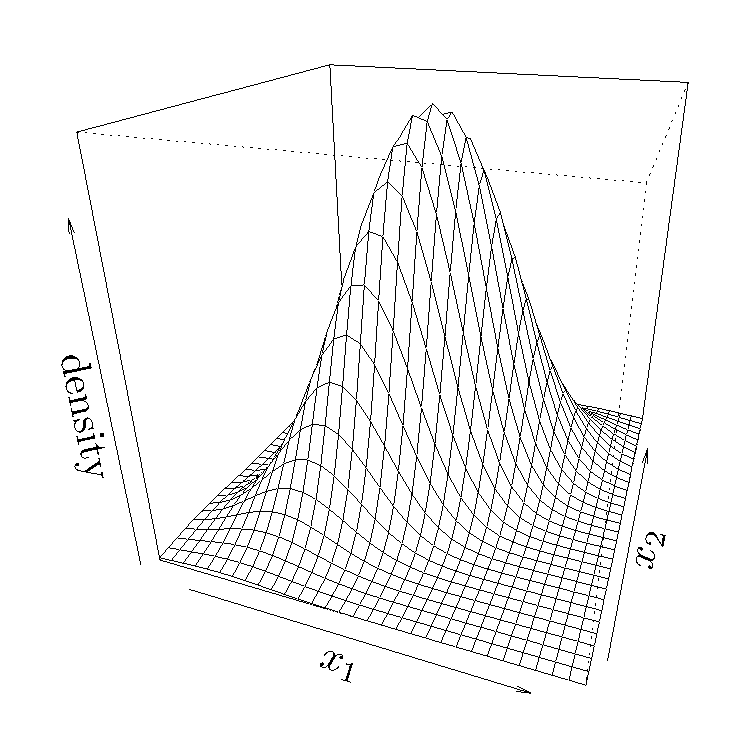
\includegraphics[height=4.7cm]{figures/R/MVN_dens2} \qquad 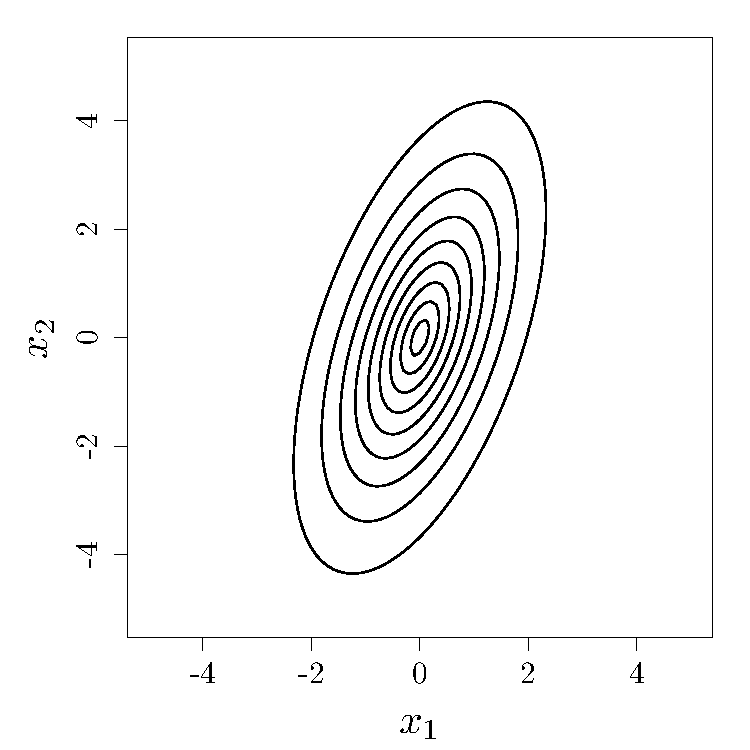
\includegraphics[height=5cm]{figures/R/ch1_pdf2} 
\end{center}
\end{frame}


%%%%%%%%%%%%%%%%%%%%%%%%%%%%%%%%%%%%%%%%%%%%%%%%%%%%%%
\begin{frame}{}
\begin{example}
\begin{center}
 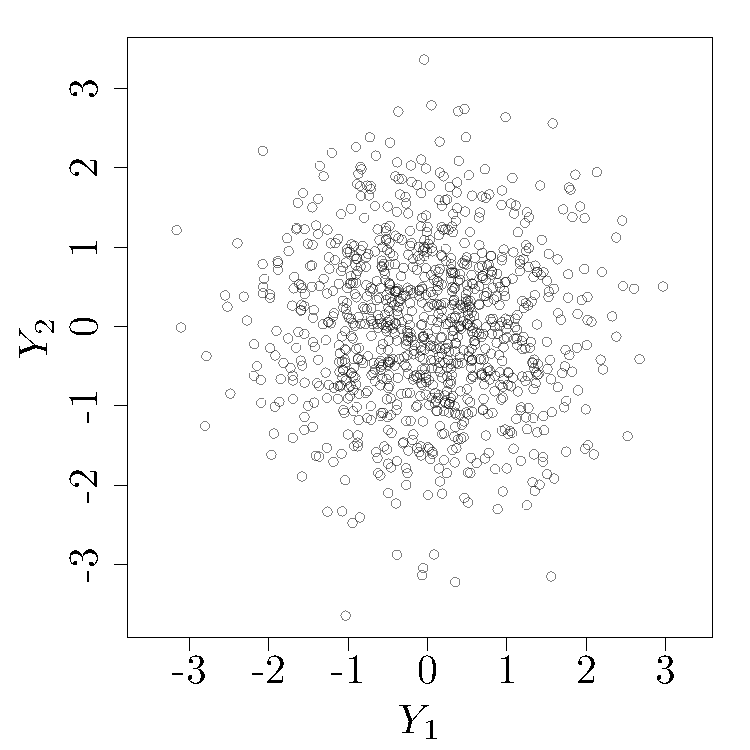
\includegraphics[height=5cm]{figures/R/MVN_gaussvec2} \quad 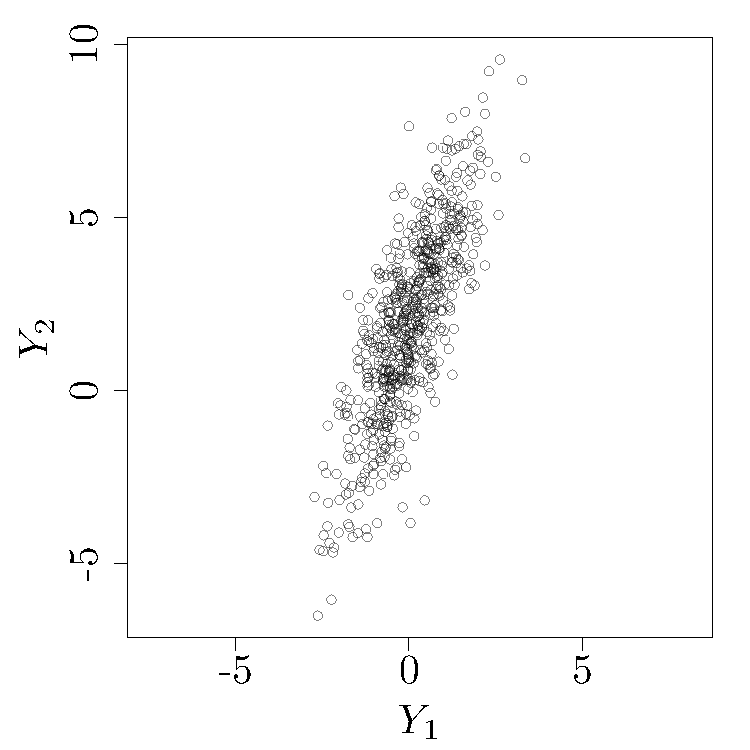
\includegraphics[height=4.5cm]{figures/R/MVN_gaussvec1} 
\end{center}
\end{example}
\end{frame}

%%%%%%%%%%%%%%%%%%%%%%%%%%%%%%%%%%%%%%%%%%%%%%%%%%%%%%
\begin{frame}{}
\begin{exampleblock}{Counter example}
\begin{center}
 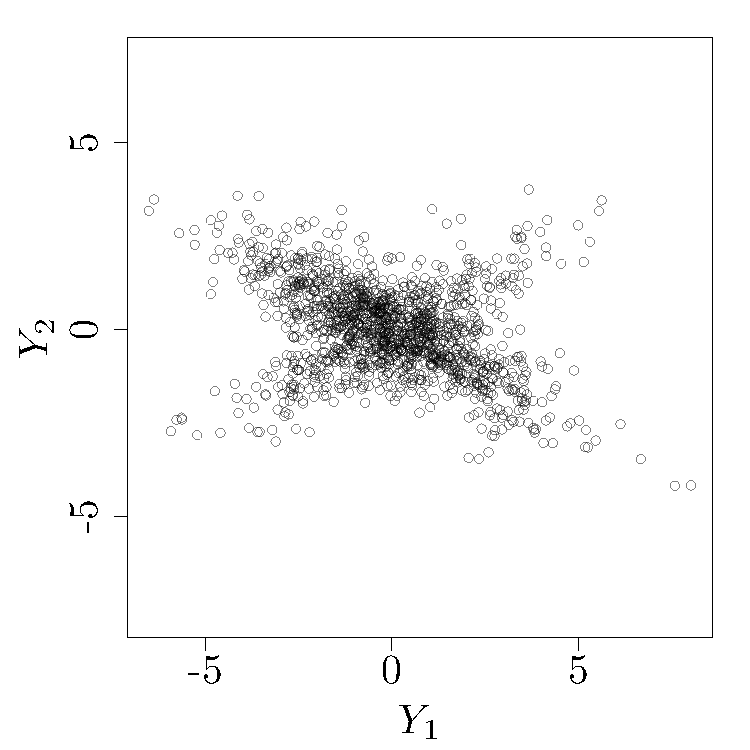
\includegraphics[height=5cm]{figures/R/MVN_gaussvec3}
\end{center}
$Y_1$ and $Y_2$ are normally distributed but \textbf{the couple $(Y_1,Y_2)$ is not}.
\end{exampleblock}
\end{frame}


%%%%%%%%%%%%%%%%%%%%%%%%%%%%%%%%%%%%%%%%%%%%%%%%%%%%%%
\begin{frame}{}
\begin{exampleblock}{Exercise}
\begin{columns}[t]
\column{5mm}
Let:
\column{9cm}
\vspace{-5.5mm}
\begin{itemize}
	\item $\varepsilon$ be a vector of $n$ independent random variables with distribution $\mathcal{N}(0,1)$. 
	\item $W$ be a matrix of size $n \times n$.
	\item $b$ be a vector of length $n$.
\end{itemize}
\end{columns}
\vspace{5mm}
We define the random vector $Y$ by 
$$ Y = W \varepsilon + b.$$
\textbf{Questions:}
\begin{enumerate}
	\item Compute the expectation of $Y$.
	\item Compute the covariance matrix of $Y$.
	\item Deduce from the above a method to generate samples from a Gaussian vector with arbitrary distribution $\mathcal{N}(\mu,\Sigma)$.
\end{enumerate}
\end{exampleblock}
\end{frame}

%%%%%%%%%%%%%%%%%%%%%%%%%%%%%%%%%%%%%%%%%%%%%%%%%%%%%%
\begin{frame}{}
\begin{block}{Conditional distribution}
Let $(Y,Z)$ be a Gaussian vector ($Y$ and $Z$ may both be vectors) with mean $(\mu_Y,\mu_Z)^t$ and covariance matrix
\begin{equation*}
\begin{pmatrix}
	\Cov(Y,Y) & \Cov(Y,Z)\\
	\Cov(Z,Y) & \Cov(Z,Z)\\
\end{pmatrix}.
\end{equation*}
The conditional distribution of $Y$ knowing $Z$ is still multivariate normal $Y|Z \sim \mathcal{N}(\mu_{cond},\Sigma_{cond})$ with
\begin{equation*}
\begin{split}
	\mu_{cond} &= \E [Y|Z] = \mu_Y + \Cov(Y,Z) \Cov(Z,Z)^{-1} (Z-\mu_Z)\\ 
	\Sigma_{cond} &= \Cov [Y,Y|Z] = \Cov(Y,Y) - \Cov(Y,Z) \Cov(Z,Z)^{-1} \Cov(Z,Y)
\end{split}
\end{equation*}
\end{block}
\end{frame}

%%%%%%%%%%%%%%%%%%%%%%%%%%%%%%%%%%%%%%%%%%%%%%%%%%%%%%
\begin{frame}{}
Here is a graphical illustration of this property:
\begin{center}
 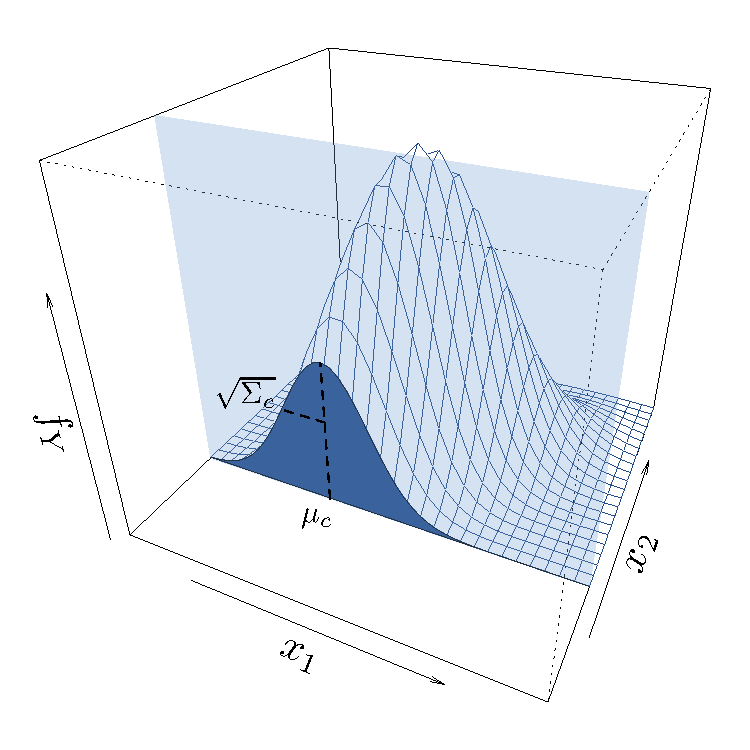
\includegraphics[height=5cm]{figures/R/ch1_condpdf1} \qquad 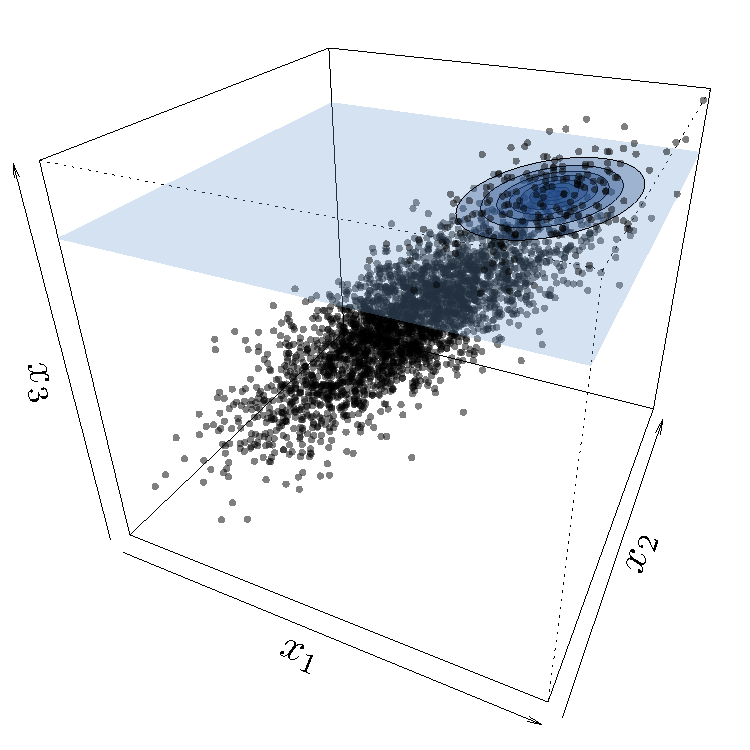
\includegraphics[height=5cm]{figures/R/ch1_condpdf2} 
\end{center}
\end{frame}

%%%%%%%%%%%%%%%%%%%%%%%%%%%%%%%%%%%%%%%%%%%%%%%%%%%%%%
\begin{frame}{}
\begin{exampleblock}{Exercise}
	Starting from the density function, prove the previous property using the Schur block inverse:
\begin{equation*}
\begin{pmatrix}
	\Sigma_{1,1} & \Sigma_{1,2}\\
	\Sigma_{2,1} & \Sigma_{2,2}\\
\end{pmatrix}^{-1} = 
\begin{pmatrix}
	A & B\\
	B^t & C\\
\end{pmatrix}
\end{equation*}
\begin{equation*}
\begin{split}
 \text{where: \quad} A &= (\Sigma_{1,1} - \Sigma_{1,2} \Sigma_{2,2}^{-1} \Sigma_{2,1})^{-1}\\
 B &= -(\Sigma_{1,1} - \Sigma_{1,2} \Sigma_{2,2}^{-1} \Sigma_{2,1})^{-1}\Sigma_{1,2}\Sigma_{2,2}^{-1}\\
 C &= \Sigma_{2,2}^{-1} + \Sigma_{2,2}^{-1} \Sigma_{2,1} (\Sigma_{1,1} -\Sigma_{1,2} \Sigma_{2,2}^{-1} \Sigma_{2,1})^{-1}\Sigma_{1,2}\Sigma_{2,2}^{-1}
\end{split}
\end{equation*}
\end{exampleblock}
\end{frame}

%%%%%%%%%%%%%%%%%%%%%%%%%%%%%%%%%%%%%%%%%%%%%%%%%%%%%%%%%%%%
%\subsection{Gaussian processes}

%%%%%%%%%%%%%%%%%%%%%%%%%%%%%%%%%%%%%%%%%%%%%%%%%%%%%%
\begin{frame}{}
The multivariate Gaussian distribution can be generalised to random processes: 
\begin{definition}
A random process $Z$ over $D \subset \mathds{R}^d$ is said to be Gaussian if 
\begin{equation*}
\forall n \in \mathds{N}, \forall x_i \in D, (Z(x_1),\dots,Z(x_n)) \text{  is a Gaussian vector}.
\end{equation*} 
\end{definition}
The distribution of a GP is fully characterised by:
\begin{itemize}
	\item its mean function $m$ defined over $D$ 
	\item its covariance function (or kernel) $k$ defined over $D \times D$: $k(x,y) = \Cov(Z(x),Z(y))$
\end{itemize}
We will use the notation $Z \sim \mathcal{N}(m(.),k(.,.))$.
\end{frame}


%%%%%%%%%%%%%%%%%%%%%%%%%%%%%%%%%%%%%%%%%%%%%%%%%%%%%%
\begin{frame}{Gaussian processes Regression}
Suppose that we have:
\begin{columns}[c]
\column{5cm}
\begin{center}
	Data\\
	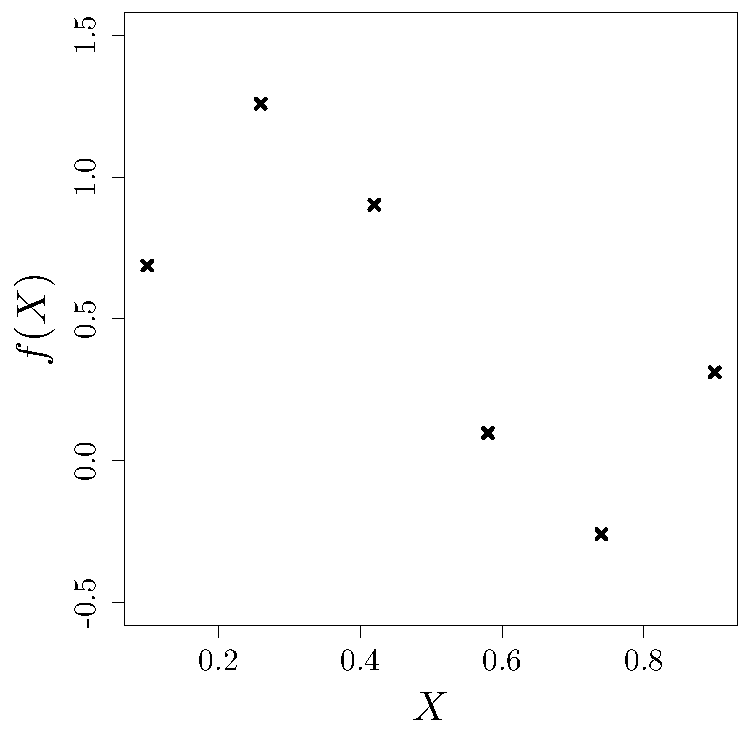
\includegraphics[height=4cm]{figures/R/GPR_obs_small}
\end{center}
\column{5cm}
\begin{center}
	$Z \sim \mathcal{N}(0,k(.,.))$\\
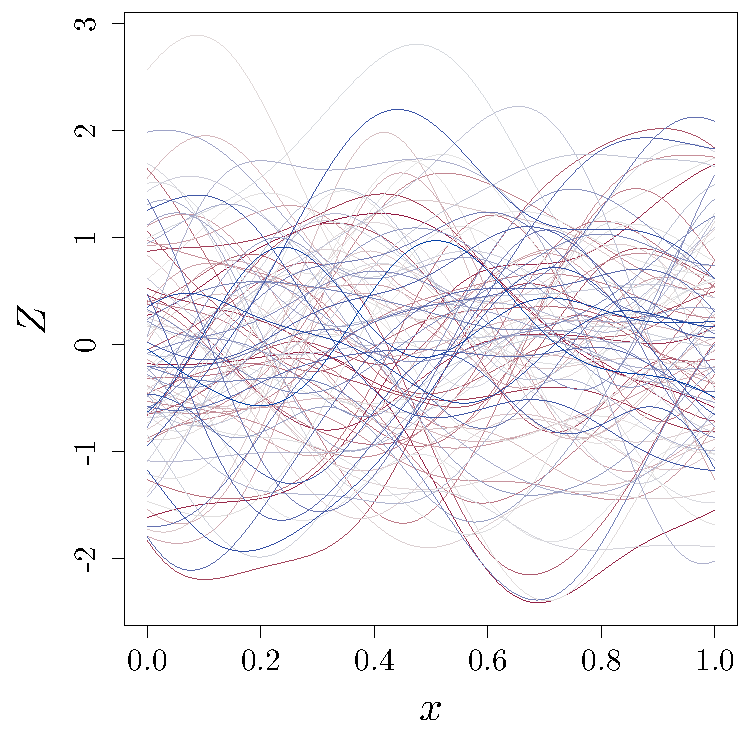
\includegraphics[height=4cm]{figures/R/GPR_simGauss}
\end{center}
\end{columns}
\begin{exampleblock}{Exercise}
\begin{itemize}
	\item[1.] What is the conditional distribution of $Z(x)|Z(X)=F$?
	\item[2.] Compute the conditional mean $m$ and covariance $c(.,.)$.
\end{itemize}
\end{exampleblock}
\end{frame}

%%%%%%%%%%%%%%%%%%%%%%%%%%%%%%%%%%%%%%%%%%%%%%%%%%%%%%
\begin{frame}{}
\begin{exampleblock}{Solution}
	\begin{itemize}
		\item[1.] The conditional distribution is Gaussian.
		\item[2.] It has mean and variance
			\begin{equation*}
			\begin{split}
				m(x) &= \E[Z(x)|Z(X) \shorteq F] \\
				&= k(x,X) k(X,X)^{-1} F \\ \vspace{3mm}
				c(x,y) &= \Cov[Z(x),Z(y)|Z(X) \shorteq F] \\
				&= k(x,y) - k(x,X) k(X,X)^{-1} k(X,y)
			\end{split}
			\end{equation*}
		\end{itemize}
\end{exampleblock}
\end{frame}

%%%%%%%%%%%%%%%%%%%%%%%%%%%%%%%%%%%%%%%%%%%%%%%%%%%%%%
\begin{frame}{}
We finally obtain
\begin{center}
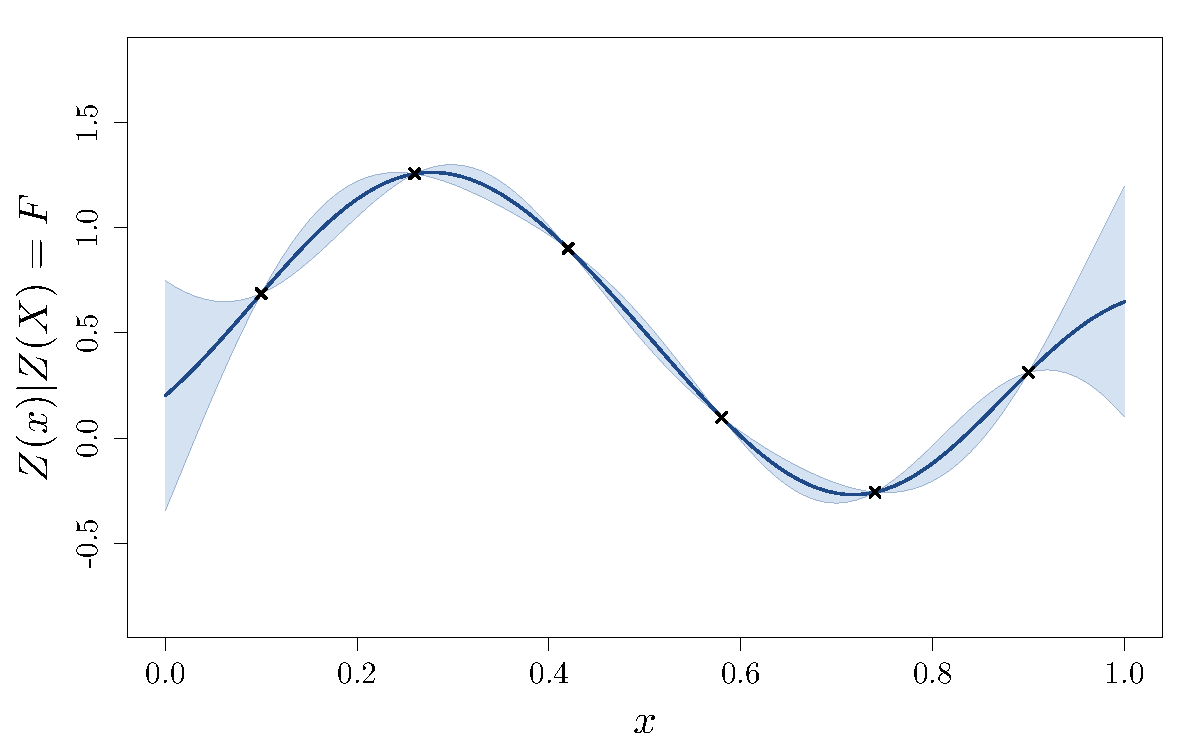
\includegraphics[height=6cm]{figures/R/GPR_GaussGPR}
\end{center}
where the blue area corresponds to $95\%$ confidence intervals: $m(x) \pm 1.96 \sqrt{c(x,x)}$. 
\end{frame}

%%%%%%%%%%%%%%%%%%%%%%%%%%%%%%%%%%%%%%%%%%%%%%%%%%%%%%
\begin{frame}{}
A few remarkable properties of GPR models 
\begin{itemize}
	\item They interpolate the data-points
	\item The prediction variance does not depend on the observations
	\item The mean predictor does not depend on the variance
	\item The mean predictor (usually) come back to zero when for predictions far away from the observations.
\end{itemize}
\vspace{5mm}
\begin{exampleblock}{Exercise}
\begin{itemize}
	\item Prove the first three items.
	\item Prove the last item for a squared exponential kernel: 
	$$k(x,y) = \exp \left(- (x-y)^2 \right).$$
\end{itemize}
\end{exampleblock}
\end{frame}

% %%%%%%%%%%%%%%%%%%%%%%%%%%%%%%%%%%%%%%%%%%%%%%%%%%%%%%
% \begin{frame}{}
% The best predictor can be seen either as a linear combination of
% \begin{itemize}
% 	\item the observations: $m(x)=\alpha^t F$
% 	\item the kernel evaluated at $X$: $m(x)=k(x,X) \beta$
% \end{itemize} 
% The later is interesting to understand the model shape and behaviour. \\
% \vspace{5mm}
% For example, we have for a squared exponential kernel
% \begin{center}
% 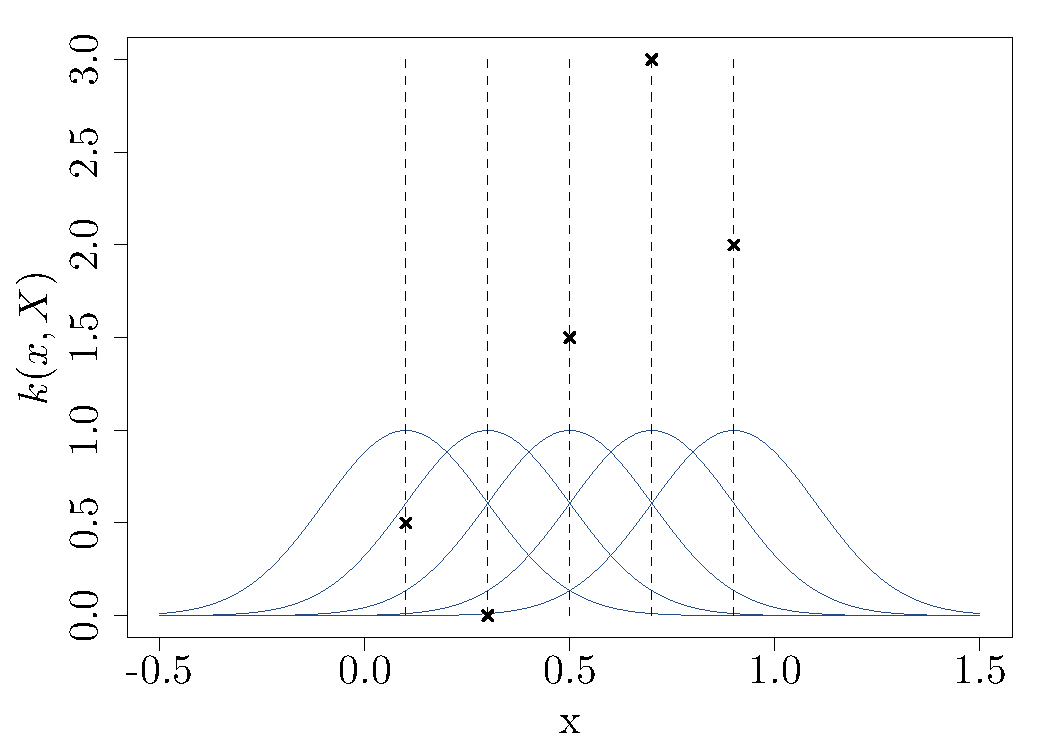
\includegraphics[height=4cm]{figures/R/ch34_basisfuncGauss}  
% 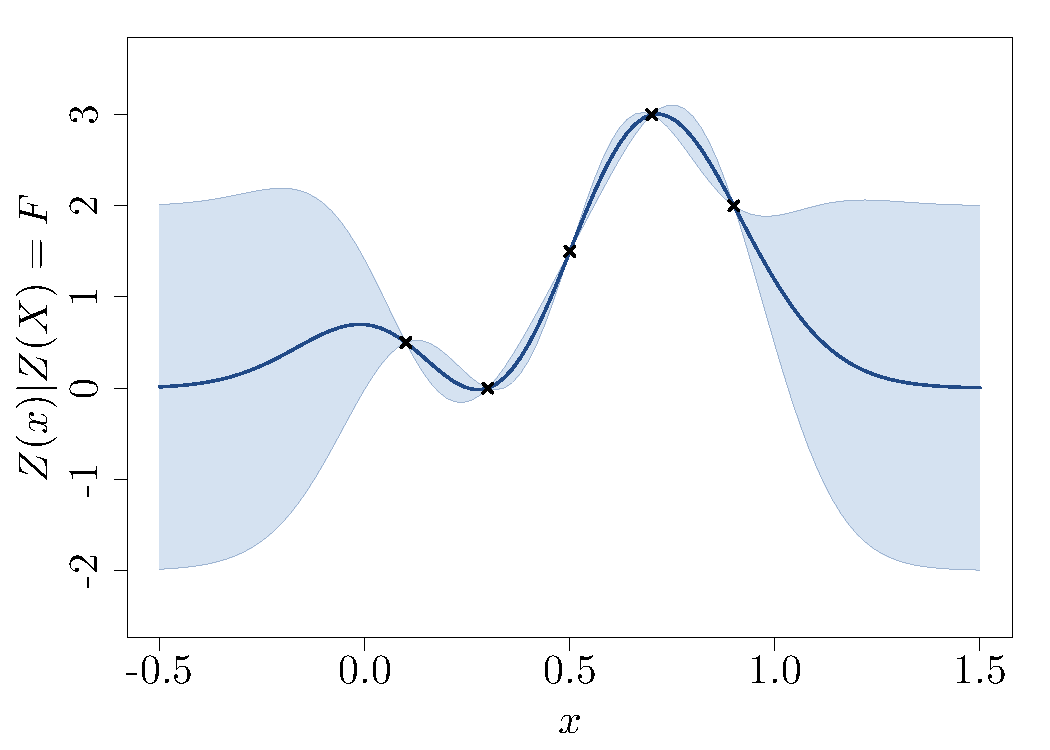
\includegraphics[height=4cm]{figures/R/ch34_GPRbasisfuncGauss} 
% \end{center}
% \end{frame}


%%%%%%%%%%%%%%%%%%%%%%%%%%%%%%%%%%%%%%%%%%%%%%%%%%%%%%%%%%%%
\section{Kernels}
\subsection{}

%%%%%%%%%%%%%%%%%%%%%%%%%%%%%%%%%%%%%%%%%%%%%%%%%%%%%%
\begin{frame}{}
For a given set of observations, the model is fully determined by the kernel.
A kernel satisfies the following properties:
\begin{itemize}
	\item It is symmetric: $k(x,y) = k(y,x)$
	\item It is positive semi-definite (psd):
\end{itemize}
\begin{equation*}
	\forall n \in \mathds{N}, \forall x_i \in D, \forall \alpha \in \mathds{R}^n,\  \sum_{i=1}^n \sum_{j=1}^n \alpha_i \alpha_j k(x_i,x_j) \geq 0
\end{equation*}
\vspace{5mm} \\
Furthermore any symmetric psd function can be seen as the covariance of a Gaussian process. This equivalence is known as the Loeve theorem.
\end{frame}

%%%%%%%%%%%%%%%%%%%%%%%%%%%%%%%%%%%%%%%%%%%%%%%%%%%%%%
\begin{frame}{}
Proving that a function is psd is often intractable. However there are a lot of functions that have already been proven to be psd:\\
\vspace{2mm}
\footnotesize
\begin{tabular}{rlN}
		constant & $ \displaystyle k(x,y) = 1 $ &\\[4mm]
		white noise & $ \displaystyle k(x,y) = \delta_{x,y} $ &\\[4mm]
		Brownian & $ \displaystyle k(x,y) =  \min (x,y) $ &\\[4mm]
		exponential & $\displaystyle k(x,y) = \exp \left(- |x-y| \right)$ &\\[4mm]
		Matern 3/2 & $\displaystyle k(x,y) = \left(1 + |x-y| \right) \exp \left(- |x-y| \right)$ &\\[4mm]
		Matern 5/2 & $\displaystyle k(x,y) = \left(1 + |x-y| + 1/3|x-y|^2 \right) \exp \left(- |x-y| \right)$ &\\[4mm]
		squared exp. & $\displaystyle k(x,y) = \exp \left(- (x-y)^2 \right)$ &\\[4mm]
		$\vdots$ & 
		% linear & $ \displaystyle k(x,y) = \sigma^2 xy $ &\\[4mm]
		% cosine & $ \displaystyle k(x,y) = \sigma^2 \cos \left (\frac{x-y}{\theta} \right) $ &\\[4mm]
		% sinc & $ \displaystyle k(x,y) = \sigma^2 \frac{\theta}{x-y} \sin \left( \frac{x-y}{\theta} \right) $ &\\[4mm] \hline
\end{tabular}\\
\vspace{2mm}
\normalsize
When $k$ is a function of $x-y$, the kernel is called \textbf{stationary}.
\end{frame}

%%%%%%%%%%%%%%%%%%%%%%%%%%%%%%%%%%%%%%%%%%%%%%%%%%%%%%
\begin{frame}{}
Changing the kernel \alert{has a huge impact on the model}:\\ 
\begin{center}
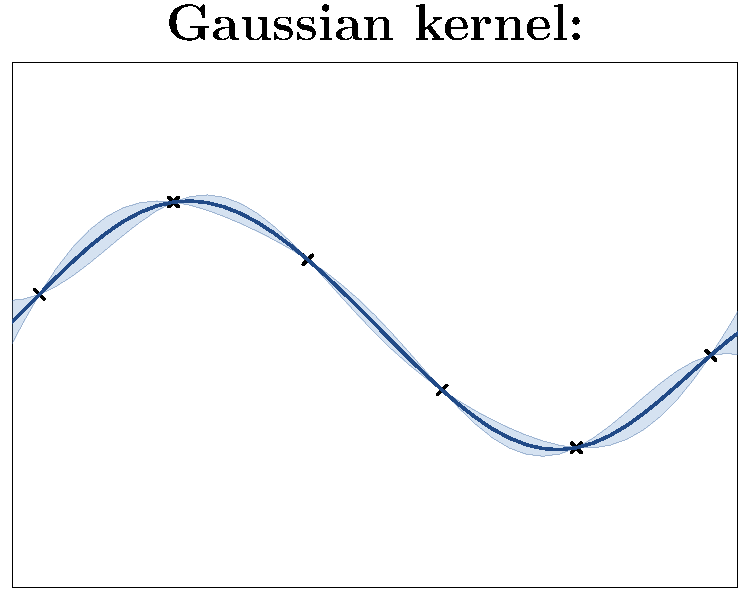
\includegraphics[height=3.9cm]{figures/R/Fig2-GP-rbf} \qquad 
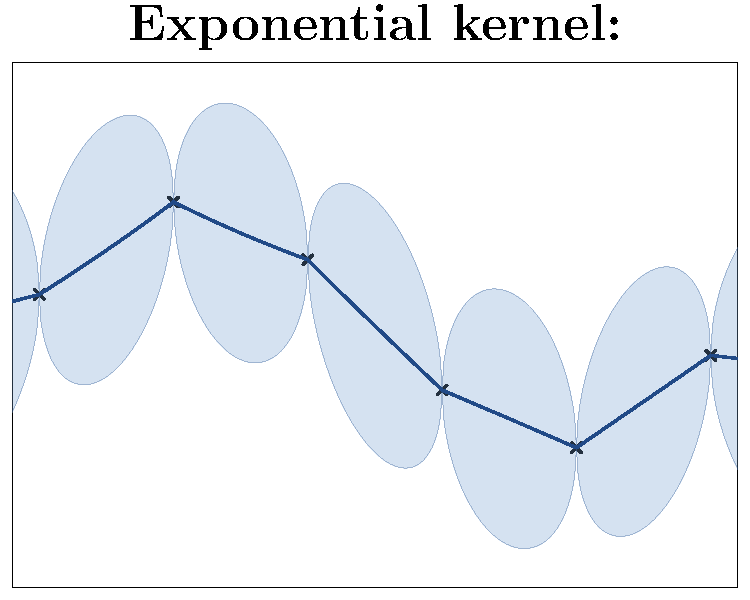
\includegraphics[height=3.9cm]{figures/R/Fig2-GP-exp}
\end{center}
\end{frame}

%%%%%%%%%%%%%%%%%%%%%%%%%%%%%%%%%%%%%%%%%%%%%%%%%%%%%%
\begin{frame}{}
This is because changing the kernel means changing the prior on $f$\\ 
\begin{center}
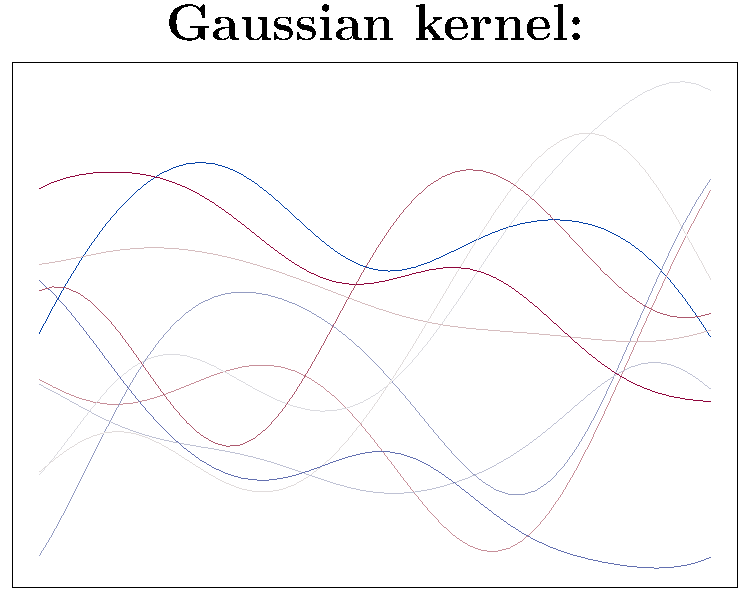
\includegraphics[height=3.8cm]{figures/R/Fig2-sim-rbf} \qquad 
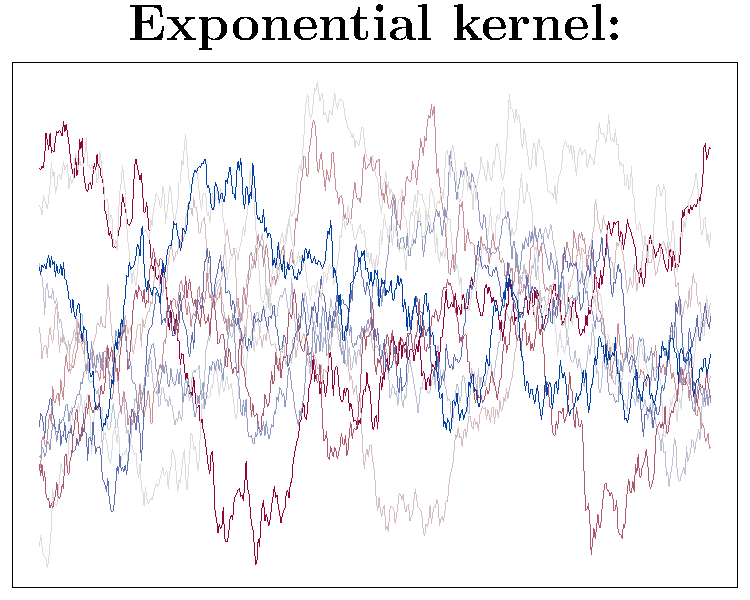
\includegraphics[height=3.8cm]{figures/R/Fig2-sim-exp}
\end{center}
\end{frame}

%%%%%%%%%%%%%%%%%%%%%%%%%%%%%%%%%%%%%%%%%%%%%%%%%%%%%%
\begin{frame}{}
There is no model/kernel that is intrinsically better... it depends on the data!
\begin{center}
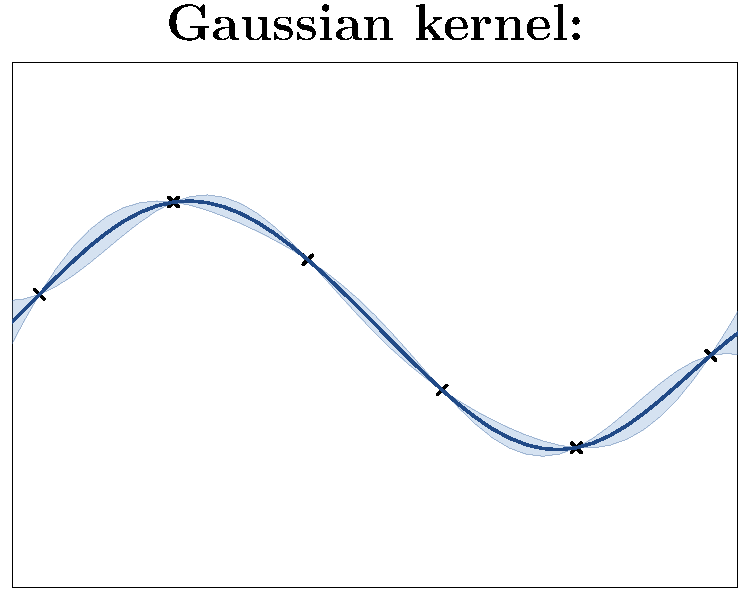
\includegraphics[height=3.5cm]{figures/R/Fig2-GP-rbf} \hspace{1cm}
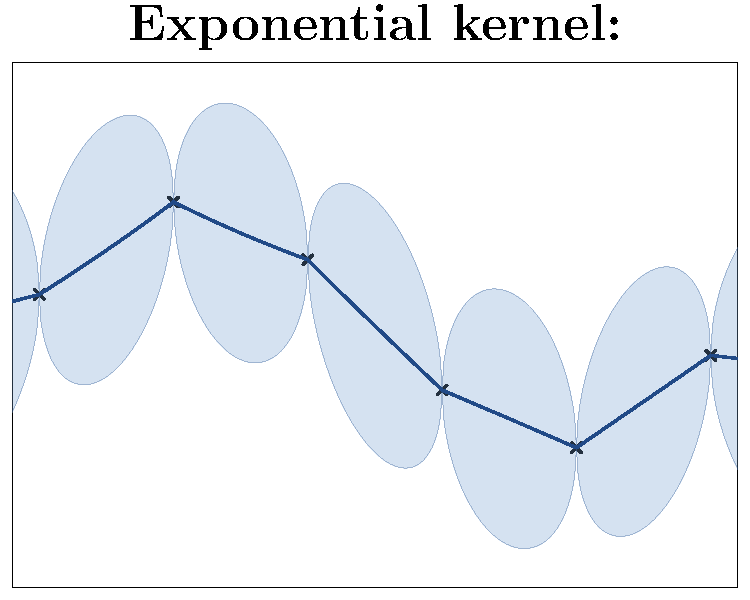
\includegraphics[height=3.5cm]{figures/R/Fig2-GP-exp}
\end{center}
The kernel has to be chosen accordingly to our prior belief on the behaviour of the function to study:
\begin{itemize}
	\item is it continuous, differentiable, how many times?
	\item is it stationary ?
	\item ...
\end{itemize}
\end{frame}


%%%%%%%%%%%%%%%%%%%%%%%%%%%%%%%%%%%%%%%%%%%%%%%%%%%%%%
\begin{frame}{}
We have seen that one kernel gives one model. However, one can include some scaling parameters into the kernels to improve their adequacy to the data:
\begin{exampleblock}{Exercise:}
If $Z$ is a GP $\mathcal{N}(0,k(.,.))$, can you detail the distribution of $Y(x) = \sigma Z(x/\theta)$
\end{exampleblock}
\vspace{5mm}
$\sigma^2$ is called the \textbf{variance} and $\theta$ the \textbf{lengthscale}
\end{frame}

%%%%%%%%%%%%%%%%%%%%%%%%%%%%%%%%%%%%%%%%%%%%%%%%%%%%%%
\begin{frame}{}
\begin{exampleblock}{Exercise: }
The kernel is Matern 5/2. Can you put each line in the right order?
\begin{center}
\begin{tabular}{ccc}
$(\sigma^2,\theta) = (3,3)$& $(\sigma^2,\theta)=(1,0.5)$& $(\sigma^2,\theta)=(1,50)$ \\ 
&&\\
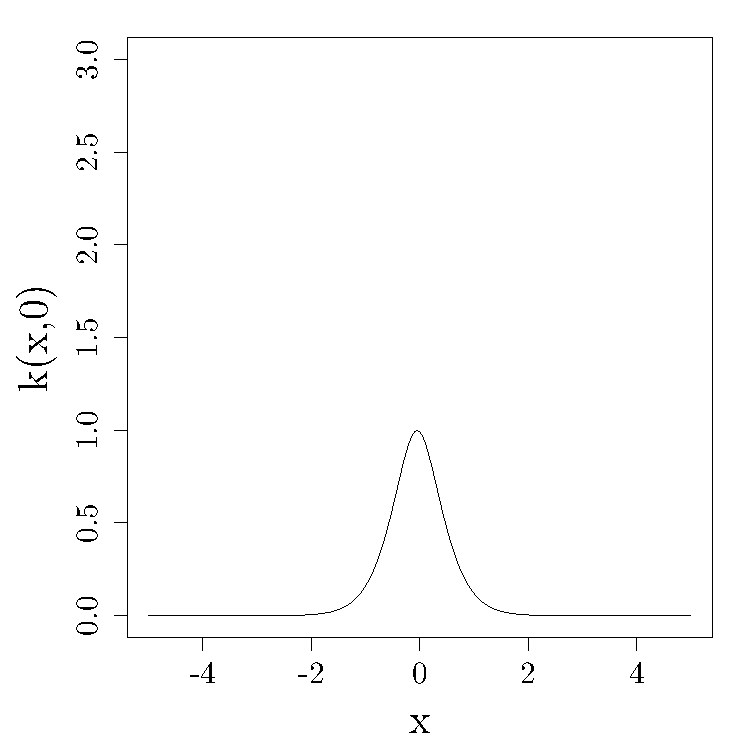
\includegraphics[height=3cm]{figures/R/MVN_kern105} &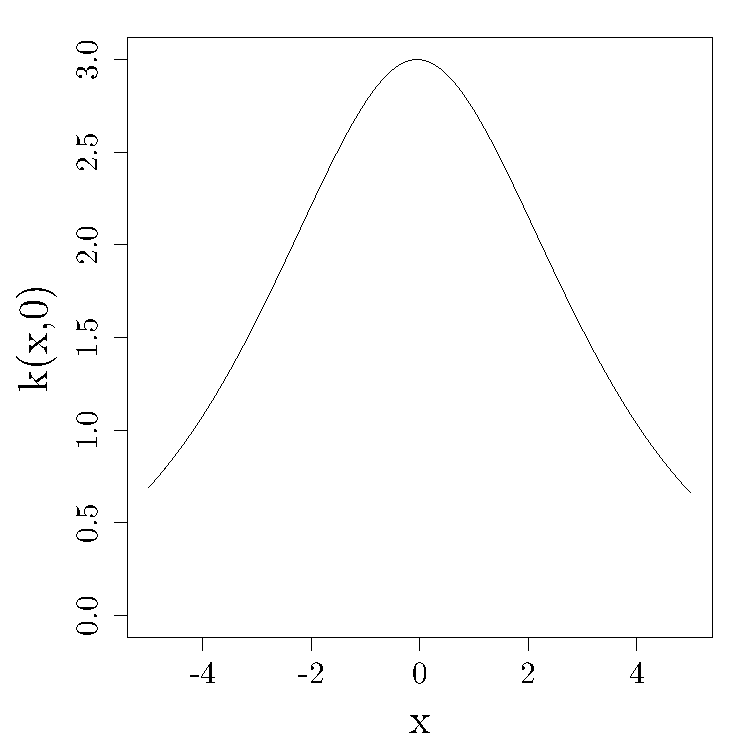
\includegraphics[height=3cm]{figures/R/MVN_kern33}& 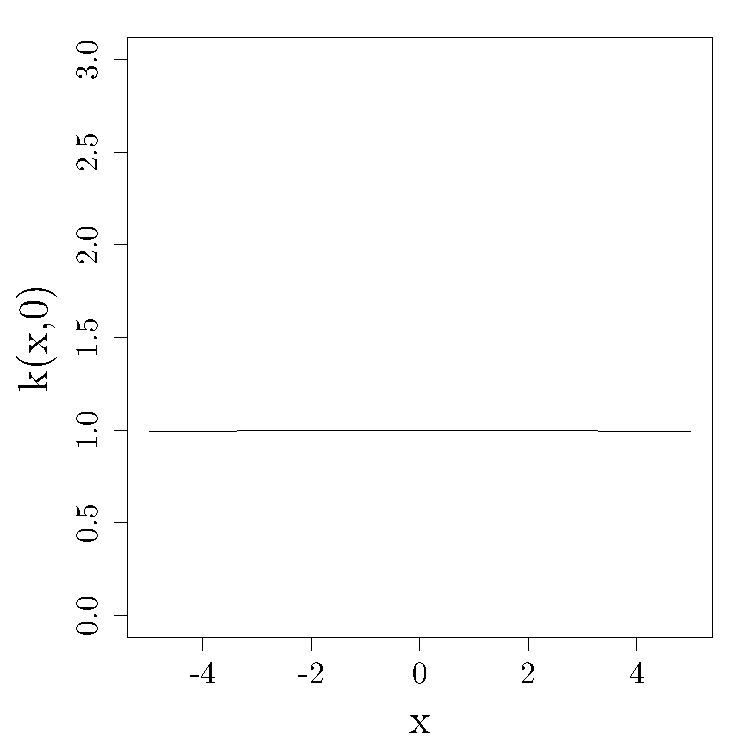
\includegraphics[height=3cm]{figures/R/MVN_kern150}\\ 
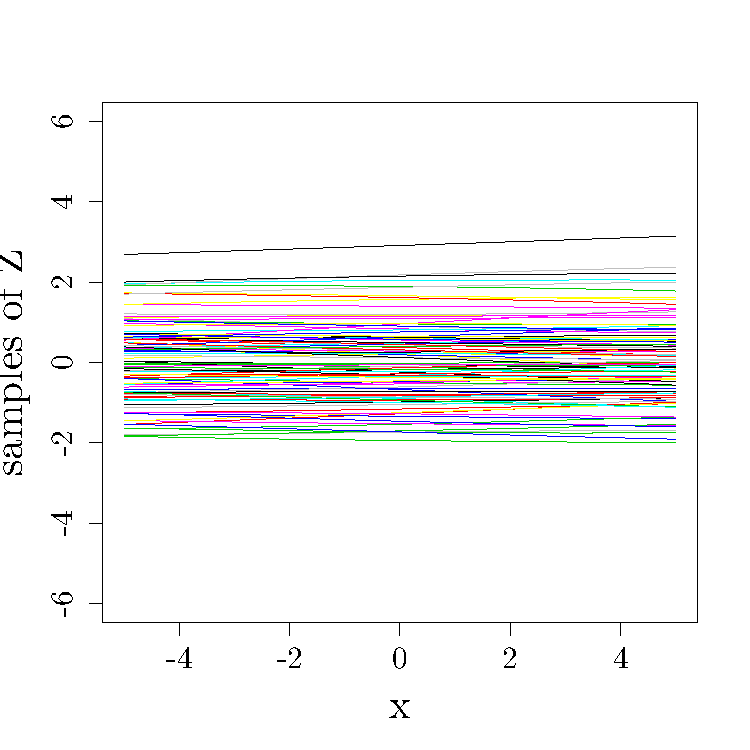
\includegraphics[height=3cm]{figures/R/MVN_traj150} &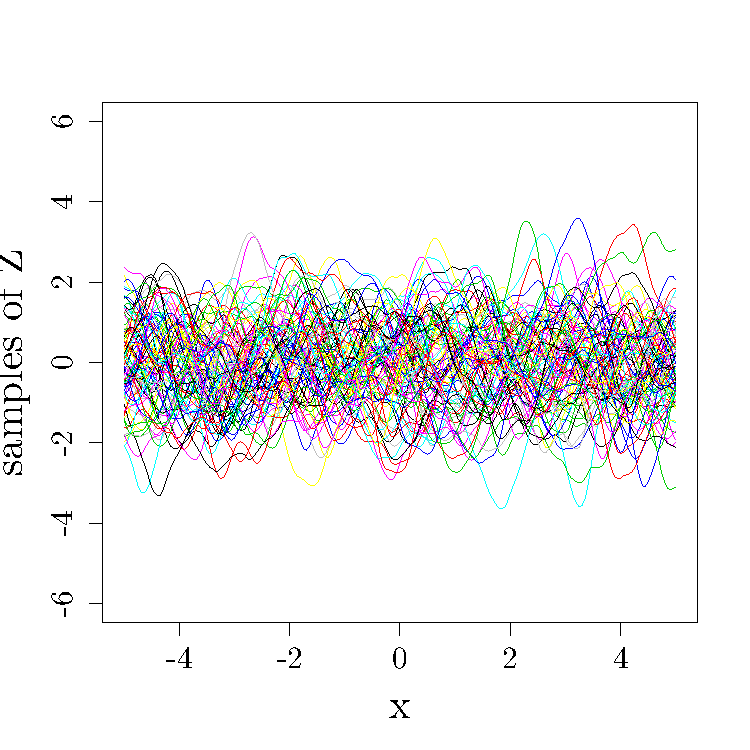
\includegraphics[height=3cm]{figures/R/MVN_traj105}& 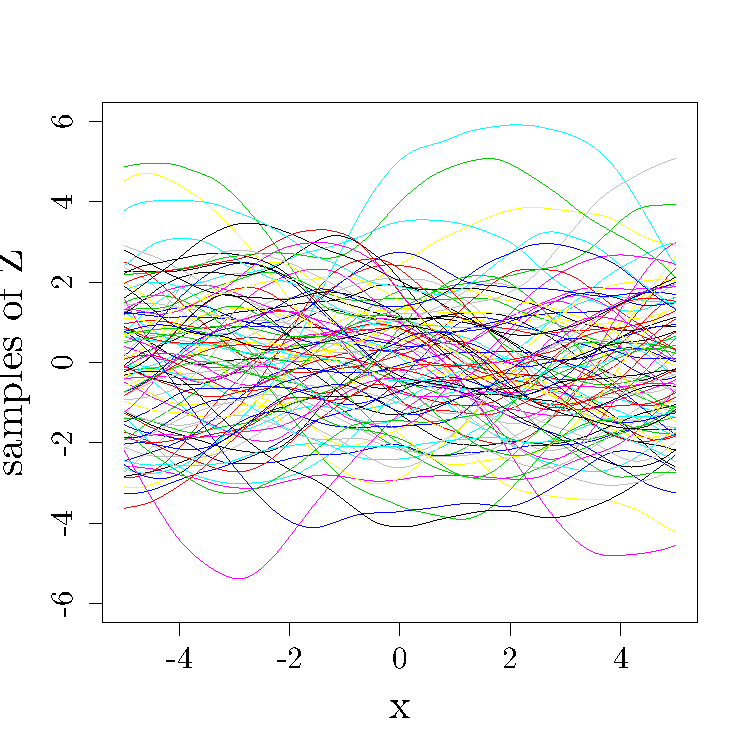
\includegraphics[height=3cm]{figures/R/MVN_traj33}
\end{tabular}
\end{center}
\end{exampleblock}
\end{frame}

%%%%%%%%%%%%%%%%%%%%%%%%%%%%%%%%%%%%%%%%%%%%%%%%%%%%%%
\begin{frame}{}
\begin{exampleblock}{Exercise: }
Answer is:
\begin{center}
\begin{tabular}{ccc}
$(\sigma^2,\theta) = (3,3)$& $(\sigma^2,\theta)=(1,0.5)$& $(\sigma^2,\theta)=(1,50)$ \\ 
&&\\
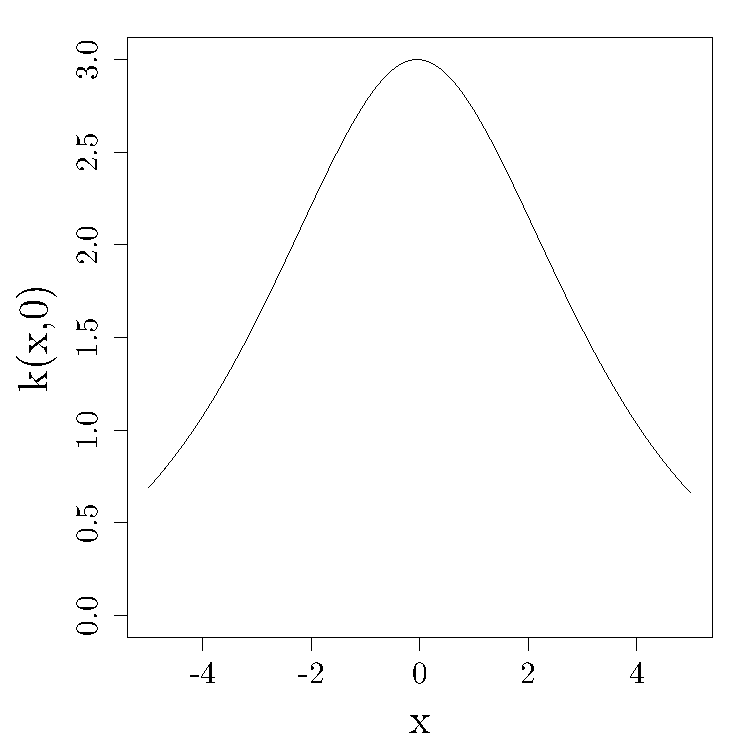
\includegraphics[height=3cm]{figures/R/MVN_kern33} &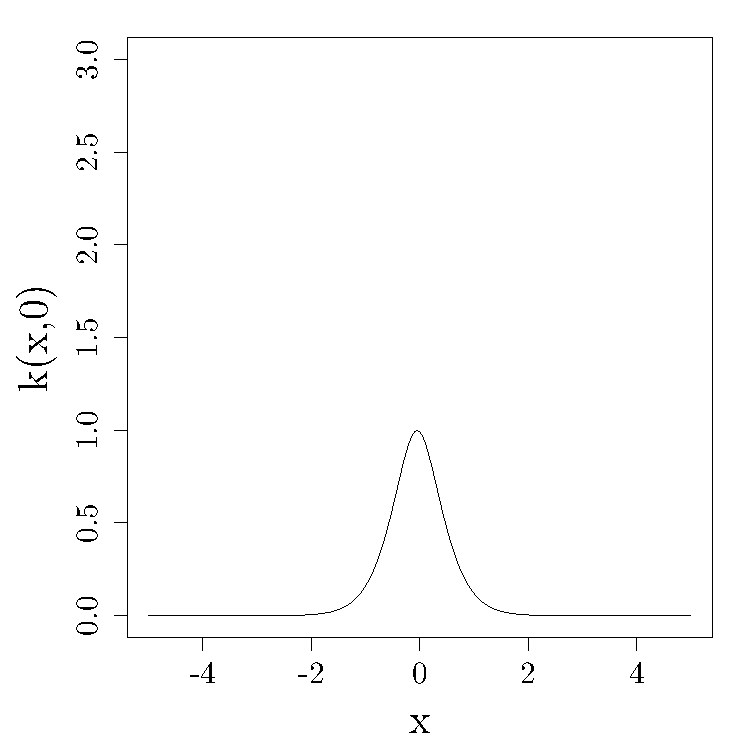
\includegraphics[height=3cm]{figures/R/MVN_kern105}& 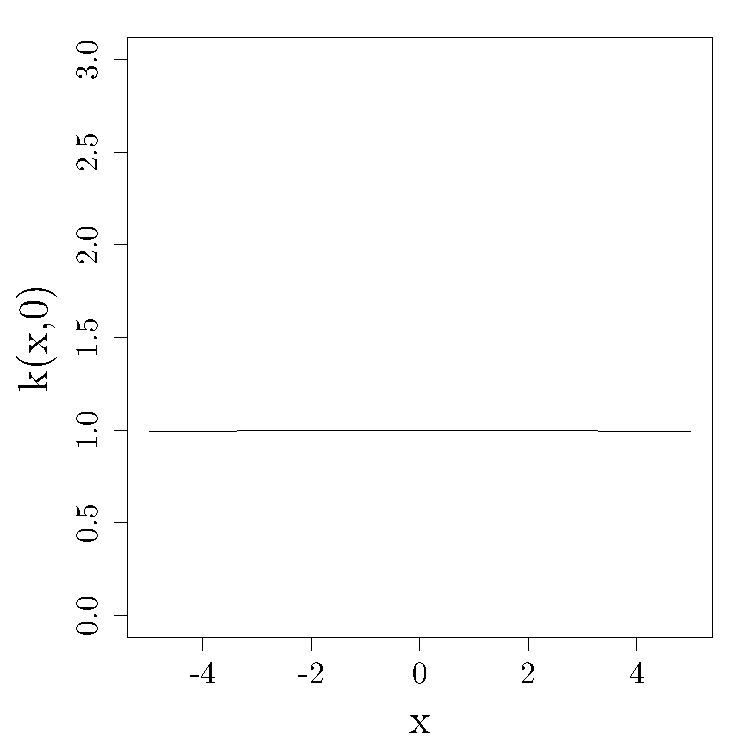
\includegraphics[height=3cm]{figures/R/MVN_kern150}\\ 
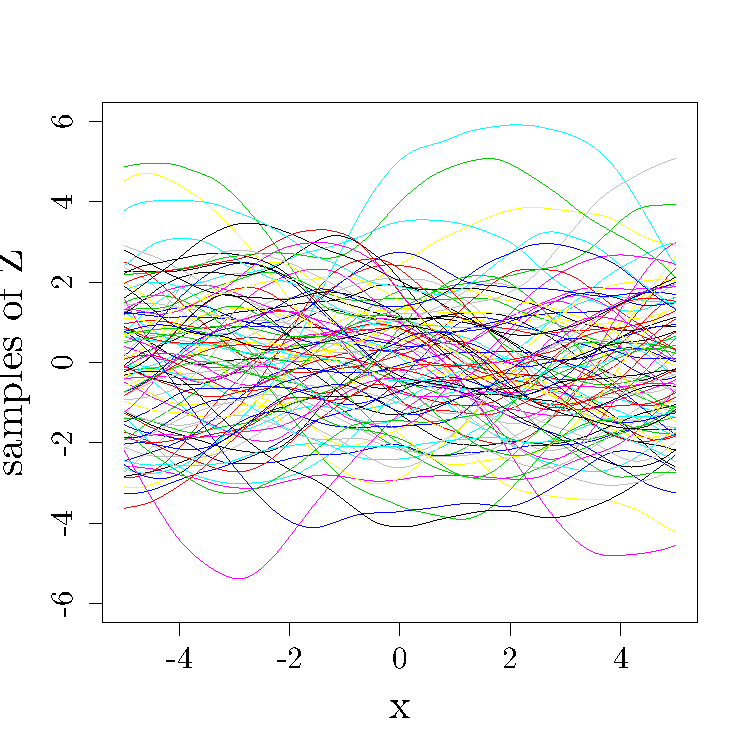
\includegraphics[height=3cm]{figures/R/MVN_traj33} &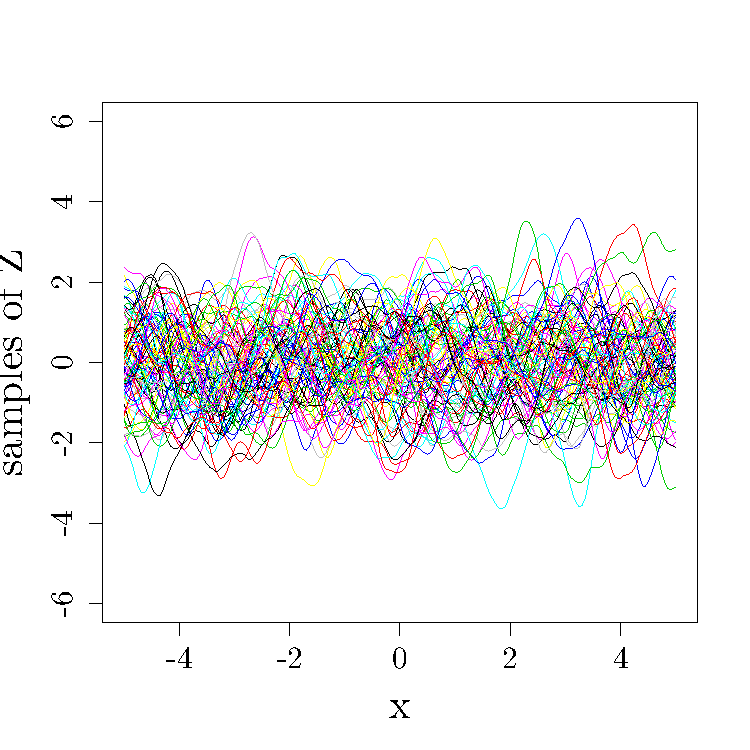
\includegraphics[height=3cm]{figures/R/MVN_traj105}& 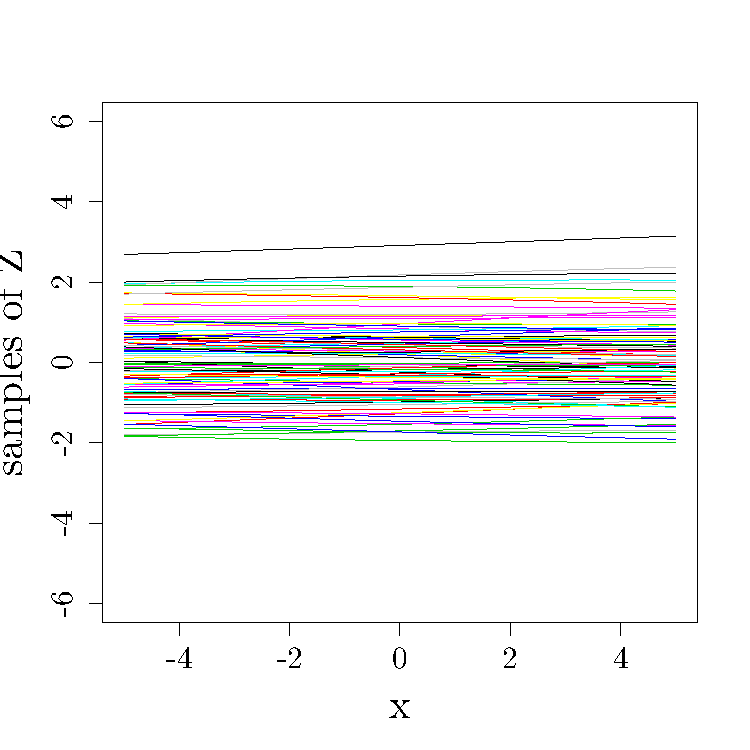
\includegraphics[height=3cm]{figures/R/MVN_traj150}
\end{tabular}
\end{center}
\end{exampleblock}
\end{frame}

% %%%%%%%%%%%%%%%%%%%%%%%%%%%%%%%%%%%%%%%%%%%%%%%%%%%%%%
% \begin{frame}{}
% Influence of the parameters on models \structure{$\Rightarrow$ lab session}
% \end{frame}

%%%%%%%%%%%%%%%%%%%%%%%%%%%%%%%%%%%%%%%%%%%%%%%%%%%%%%
\begin{frame}{}
Adding these parameters to usual kernels gives\\
\vspace{2mm}
\footnotesize
\begin{tabular}{rlN}
		squared exp. & $\displaystyle k(x,y) = \sigma^2 \exp \left(- \frac{(x-y)^2}{2 \theta^2} \right)$ &\\[6mm]
		Matern 5/2 & $\displaystyle k(x,y) = \sigma^2 \left(1 + \frac{\sqrt{5}|x-y|}{\theta} + \frac{5|x-y|^2}{3 \theta^2} \right) \exp \left(- \frac{\sqrt{5}|x-y|}{\theta} \right)$ &\\[6mm]
		Matern 3/2 & $\displaystyle k(x,y) = \sigma^2 \left(1 + \frac{\sqrt{3}|x-y|}{\theta} \right) \exp \left(- \frac{\sqrt{3}|x-y|}{\theta} \right)$ &\\[6mm]
		exponential & $\displaystyle k(x,y) = \sigma^2 \exp \left(- \frac{|x-y|}{\theta} \right)$ &\\[6mm]
		Brownian & $ \displaystyle k(x,y) = \sigma^2 \min (x,y) $ &\\[6mm]
		white noise & $ \displaystyle k(x,y) = \sigma^2 \delta_{x,y} $ &\\[6mm]
		constant & $ \displaystyle k(x,y) = \sigma^2 $ &\\[6mm]
		linear & $ \displaystyle k(x,y) = \sigma^2 xy $ &\\[6mm]
\end{tabular}
\end{frame}

%%%%%%%%%%%%%%%%%%%%%%%%%%%%%%%%%%%%%%%%%%%%%%%%%%%%%%
\begin{frame}{}
For $d \geq 2$, there can be one rescaling parameter per dimension:
\begin{equation*}
	\N{x-y}{\theta} = \left( \sum_{i=1}^d \frac{(x_i-y_i)^2}{\theta_i^2} \right)^{1/2}.
\end{equation*}
\vspace{2mm}
\footnotesize
\begin{tabular}{rlN}
        squared exp. & $\displaystyle k(x,y) = \sigma^2 \exp \left(- \frac12 \N{x-y}{\theta}^2 \right)$ &\\[6mm]
        Matern 5/2 & $\displaystyle k(x,y) = \sigma^2 \left(1 + \sqrt{5}\N{x-y}{\theta} + \frac{5}{3}\N{x-y}{\theta}^2 \right) \exp \left(- \sqrt{5}\N{x-y}{\theta} \right)$ &\\[6mm]
        Matern 3/2 & $\displaystyle k(x,y) = \sigma^2 \left(1 + \sqrt{3}\N{x-y}{\theta} \right) \exp \left(- \sqrt{3}\N{x-y}{\theta}  \right)$ &\\[6mm]
        exponential & $\displaystyle k(x,y) = \sigma^2 \exp \left(- \N{x-y}{\theta} \right)$ 
\end{tabular}
\normalsize
\\ \vspace{5mm} \
If all $\theta_i$ are equal, we say that the kernel/process is \textbf{isotropic}.
\end{frame}

%%%%%%%%%%%%%%%%%%%%%%%%%%%%%%%%%%%%%%%%%%%%%%%%%%%%%%
%%%%%%%%%%%%%%%%%%%%%%%%%%%%%%%%%%%%%%%%%%%%%%%%%%%%%%
\section{Parameter estimation}
\subsection{}

%%%%%%%%%%%%%%%%%%%%%%%%%%%%%%%%%%%%%%%%%%%%%%%%%%%%%%
\begin{frame}{}
We have seen previously that the choice of the kernel and its parameters have a great influence on the model. \\ \vspace{5mm}
In order to choose a prior that is suited to the data at hand, we can consider:
\begin{itemize}
	\item minimising the model error
	\item Using maximum likelihood estimation 
\end{itemize}
We will now detail the second one.
\end{frame}

%%%%%%%%%%%%%%%%%%%%%%%%%%%%%%%%%%%%%%%%%%%%%%%%%%%%%%
\begin{frame}{}
The likelihood quantifies the adequacy between a distribution and some observations. 
\begin{definition}
Let $f_Y$ be a pdf depending on some parameters $p$ and let $y_1,\dots,y_n$ be independent observations. The \textbf{likelihood} is defined as 
\begin{equation*}
 	L(p) = \prod_{i=1}^n f_Y(y_i;p).
\end{equation*} 
\end{definition}
A high value of $L(p)$ indicates the observations are likely to be drawn from $f_Y(.;p)$.
\end{frame}

%%%%%%%%%%%%%%%%%%%%%%%%%%%%%%%%%%%%%%%%%%%%%%%%%%%%%%
\begin{frame}{}
In the GPR context, we often have only \textbf{one observation} of the vector $F$. The likelihood is then:
\footnotesize
\begin{equation*}
 	L(\sigma^2,\theta)= f_{Z(X)}(F;\sigma^2,\theta) = \frac{1}{\displaystyle | 2 \pi k(X,X)|^{1/2}} \exp \left(-\frac12 F^t k(X,X)^{-1} F  \right).
\end{equation*} 
\normalsize
It is thus possible to maximise $L$  with respect to the kernel's parameters in order to find a well suited prior. In practice, it is common to work with the concentrated log-likelihood:
\begin{equation*}
 	\ell (\sigma^2, \theta) =  \log(|k(X,X)|) + F^t k(X,X)^{-1} F
\end{equation*} 
The value of $\sigma^2$ can be obtained analytically. Others, such as $\theta$, need numerical optimization.
\end{frame}

%%%%%%%%%%%%%%%%%%%%%%%%%%%%%%%%%%%%%%%%%%%%%%%%%%%%%%
\begin{frame}{}
\begin{example}
	We consider 100 sample from a  Matern 5/2 process with parameters $\sigma^2=1$ and $\theta = 0.2$, and $n$ observation points. We then try to recover the kernel parameters using MLE.\\ \vspace{5mm}
	\centering
	\begin{tabular}{|c|cccc|}
		\hline
		$n$ & 5 & 10 & 15 & 20 \\ \hline
		$\sigma^2$ & 1.0 (0.7) & 1.11 (0.71) & 1.03 (0.73) & 0.88 (0.60) \\
		$\theta$ & 0.20 (0.13) & 0.21 (0.07) & 0.20 (0.04) & 0.19 (0.03) \\ \hline
	\end{tabular}
\end{example}
\vspace{5mm}
MLE can be applied regardless to the dimension of the input space.
\end{frame}


%%%%%%%%%%%%%%%%%%%%%%%%%%%%%%%%%%%%%%%%%%%%%%%%%%%%%%
%%%%%%%%%%%%%%%%%%%%%%%%%%%%%%%%%%%%%%%%%%%%%%%%%%%%%%
\section{Model validation}
\subsection{}

%%%%%%%%%%%%%%%%%%%%%%%%%%%%%%%%%%%%%%%%%%%%%%%%%%%%%%
\begin{frame}{}
We have seen that given some observations $F=f(X)$, it is very easy to build lots of models, either by changing the kernel parameters or the kernel itself.\\ \vspace{5mm}
The interesting question now is to know how to get a good model. To do so, we will need to answer the following questions:
\begin{itemize}
	\item What is a good model?
	\item How to measure it?
\end{itemize}
\end{frame}

%%%%%%%%%%%%%%%%%%%%%%%%%%%%%%%%%%%%%%%%%%%%%%%%%%%%%%
\begin{frame}{}
The idea is to introduce new data and to compare the model prediction with reality 
\begin{center}
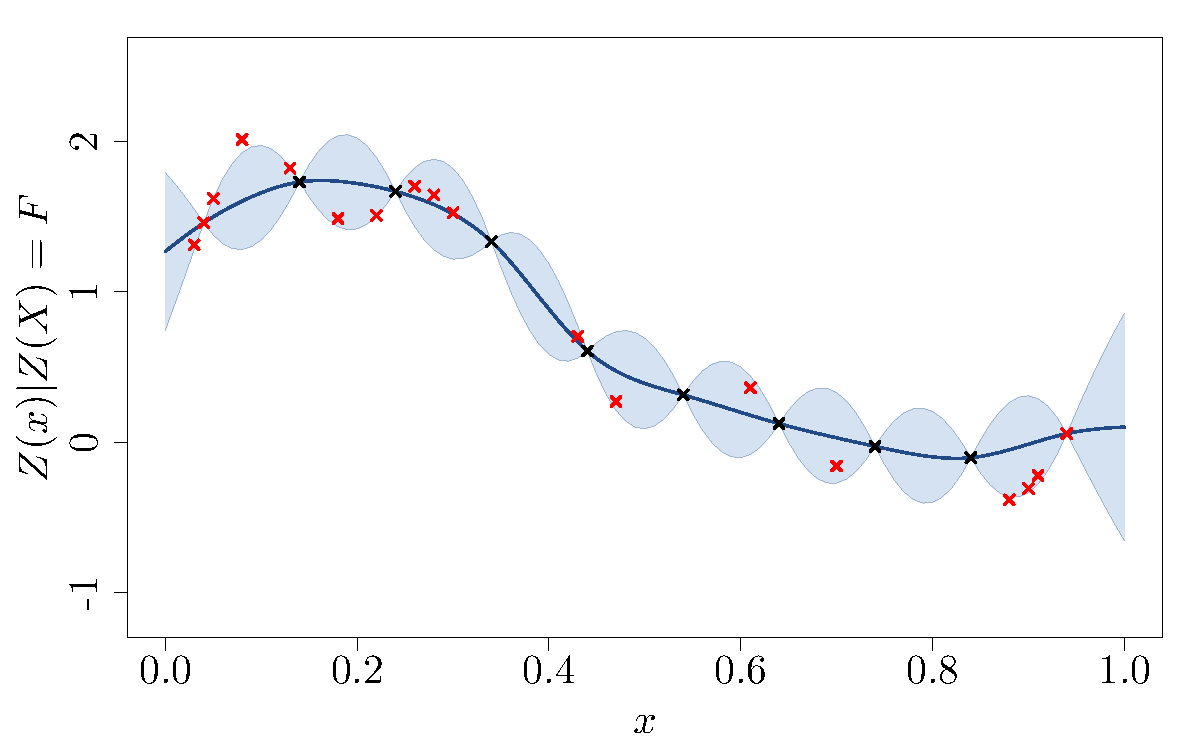
\includegraphics[height=4.5cm]{figures/R/VALID_testset}
\end{center}
\vspace{3mm}
Since GPR models provide a mean and a covariance structure for the error they both have to be assessed.
\end{frame}

%%%%%%%%%%%%%%%%%%%%%%%%%%%%%%%%%%%%%%%%%%%%%%%%%%%%%%
\begin{frame}{}
Let $X_t$ be the test set and $F_t=f(X_t)$ be the associated observations.\\ \vspace{5mm}
The accuracy of the mean can be measured by computing: 
\begin{equation*}
	\begin{split}
		\text{Mean Square Error\qquad}& MSE = \mathrm{mean} ((F_t - m(X_t))^2) \\
		\text{A ``normalised'' criterion\qquad}& Q_2 = 1 - \frac{\sum (F_t - m(X_t))^2}{\sum (F_t - \mathrm{mean}(F_t))^2} 
	\end{split}
\end{equation*}
\\ \ \\
On the above example we get $MSE = 0.038$ and $Q_2 = 0.95$.
\end{frame}

%%%%%%%%%%%%%%%%%%%%%%%%%%%%%%%%%%%%%%%%%%%%%%%%%%%%%%
\begin{frame}{}
The predicted distribution can be tested by normalising the residuals. \\ \vspace{3mm}
According to the model, $F_t \sim \mathcal{N}(m(X_t),c(X_t,X_t))$.\\ \vspace{3mm}
$c(X_t,X_t)^{-1/2}(F_t-m(X_t)) $ should thus be independents $\mathcal{N}(0,1)$:
\begin{center}
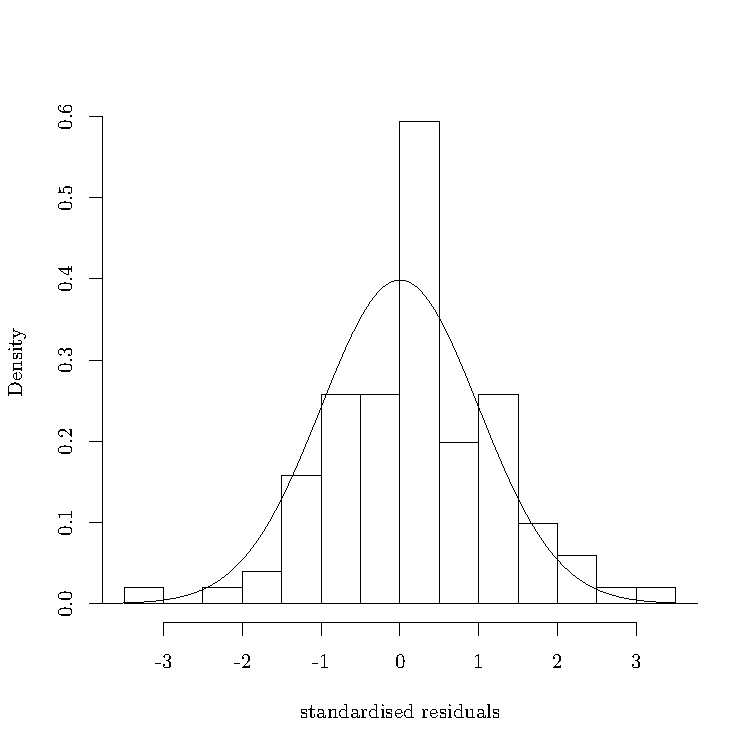
\includegraphics[height=5cm]{figures/R/VALID_hist} \qquad
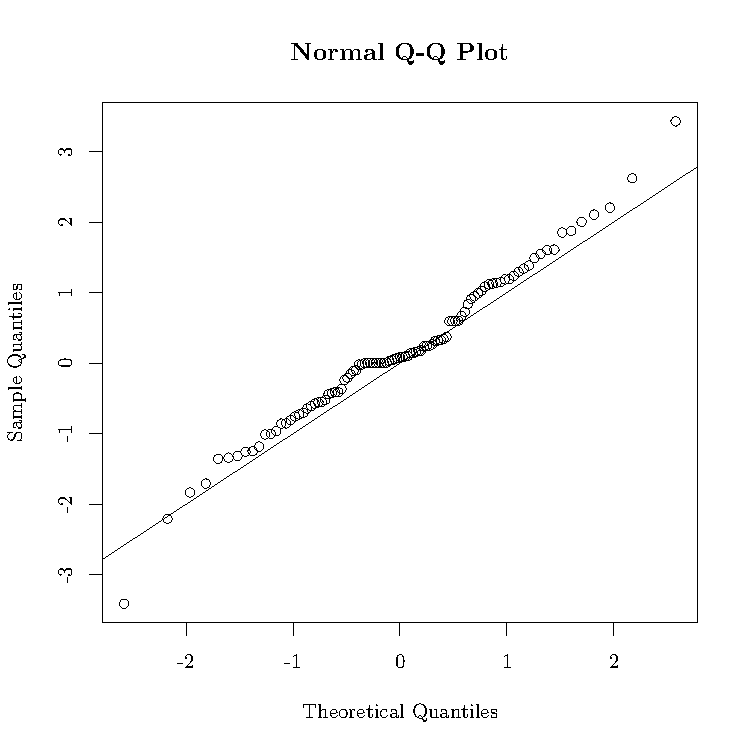
\includegraphics[height=5cm]{figures/R/VALID_qqplot}
\end{center}
\end{frame}

%%%%%%%%%%%%%%%%%%%%%%%%%%%%%%%%%%%%%%%%%%%%%%%%%%%%%%
\begin{frame}{}
When no test set is available, another option is to consider cross validation methods such as leave-one-out. \\ \vspace{5mm}
The steps are:
\begin{enumerate}
	\item[1.] build a model based on all observations except one
	\item[2.] compute the model error at this point
\end{enumerate}
This procedure can be repeated for all the design points in order to get a vector of error.
\end{frame}

%%%%%%%%%%%%%%%%%%%%%%%%%%%%%%%%%%%%%%%%%%%%%%%%%%%%%%
\begin{frame}{}
Model to be tested:\\ \vspace{3mm}
\begin{center}
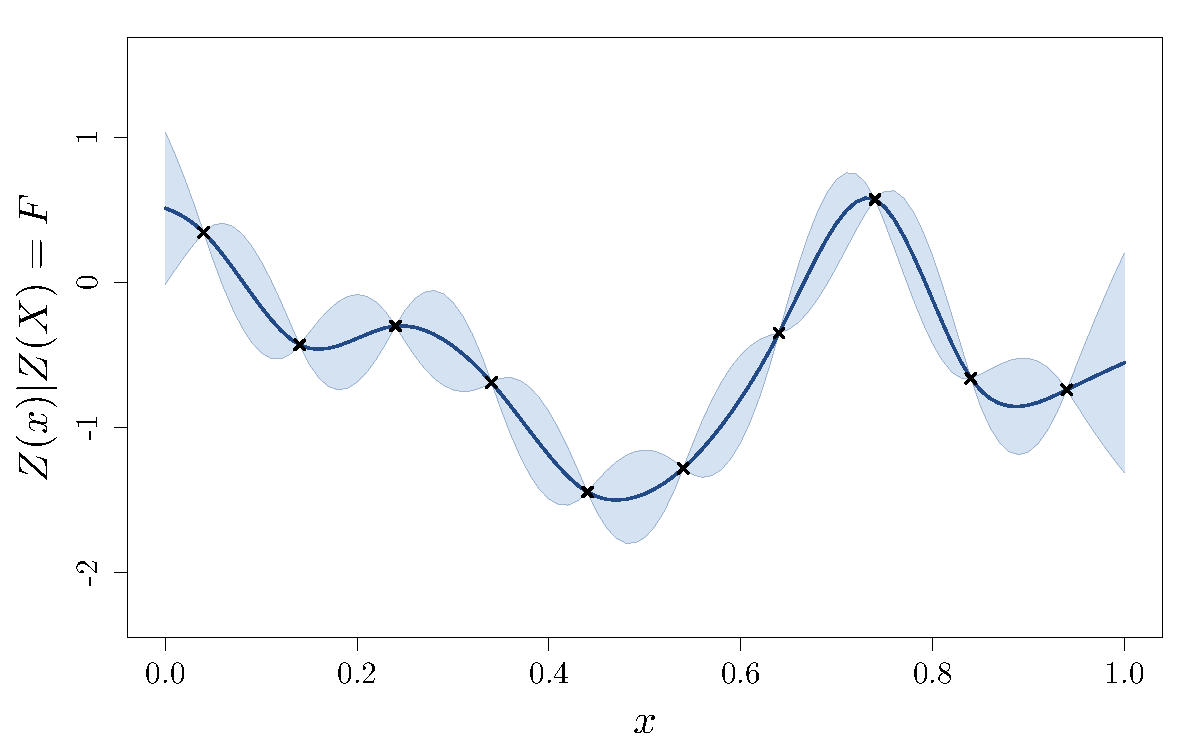
\includegraphics[height=6cm]{figures/R/VALID_crossval0}
\end{center}
\end{frame}

%%%%%%%%%%%%%%%%%%%%%%%%%%%%%%%%%%%%%%%%%%%%%%%%%%%%%%
\begin{frame}{}
Step 1:\\ \vspace{3mm}
\begin{center}
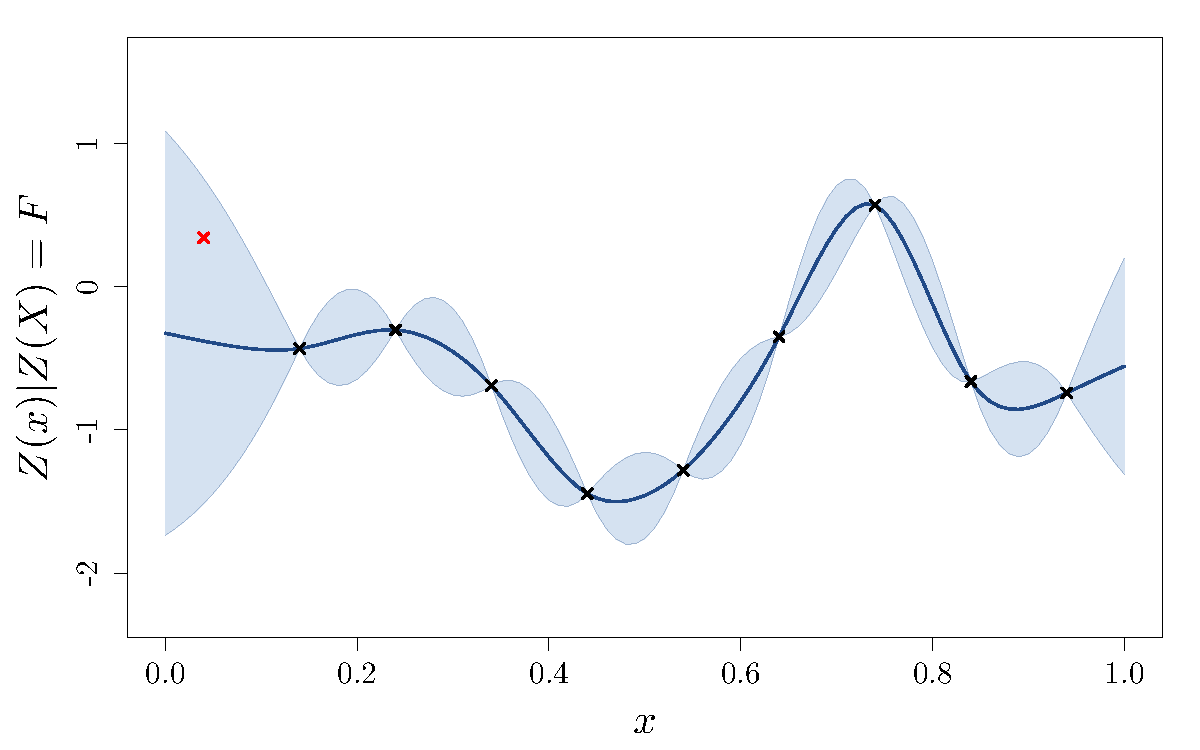
\includegraphics[height=6cm]{figures/R/VALID_crossval1}
\end{center}
\end{frame}

%%%%%%%%%%%%%%%%%%%%%%%%%%%%%%%%%%%%%%%%%%%%%%%%%%%%%%
\begin{frame}{}
Step 2:\\ \vspace{3mm}
\begin{center}
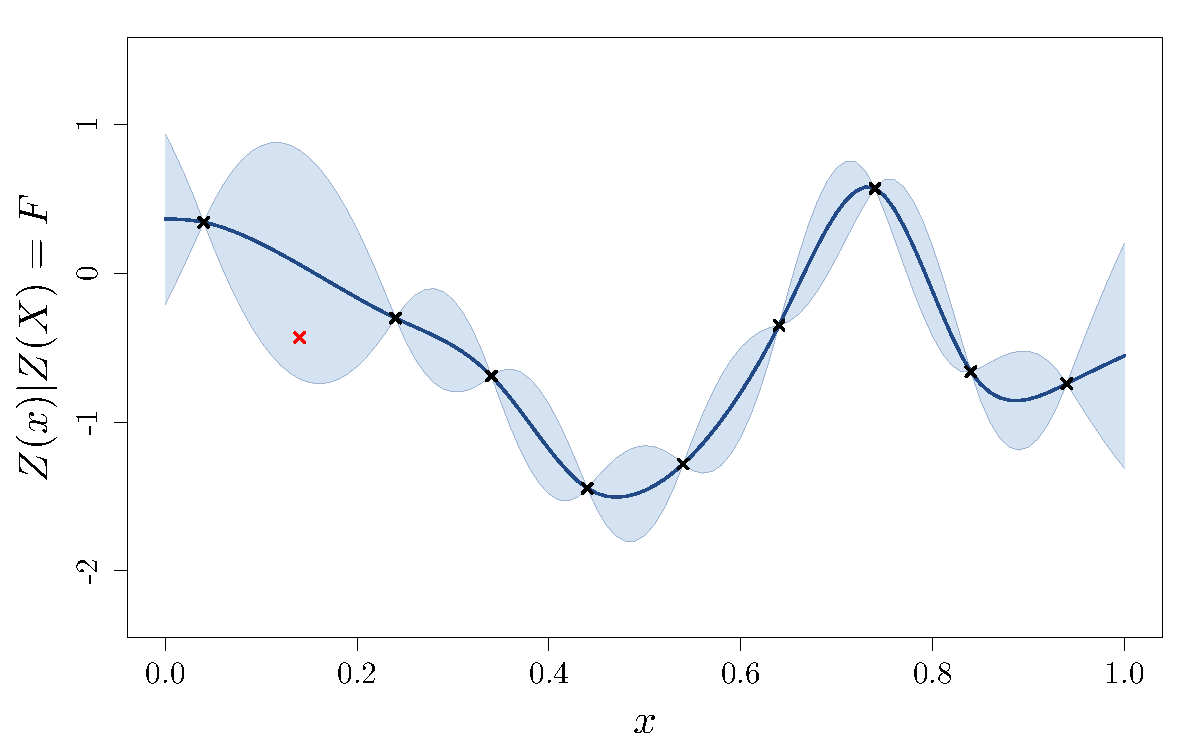
\includegraphics[height=6cm]{figures/R/VALID_crossval2}
\end{center}
\end{frame}

%%%%%%%%%%%%%%%%%%%%%%%%%%%%%%%%%%%%%%%%%%%%%%%%%%%%%%
\begin{frame}{}
Step 3:\\ \vspace{3mm}
\begin{center}
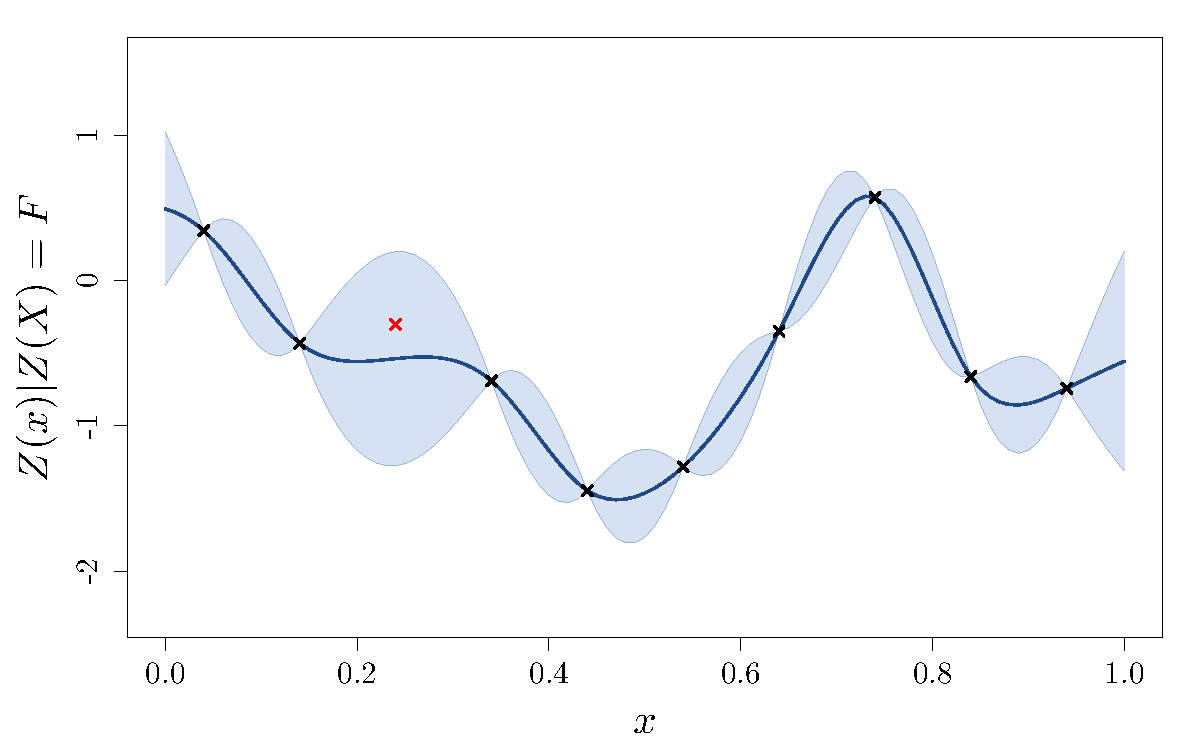
\includegraphics[height=6cm]{figures/R/VALID_crossval3}
\end{center}
\end{frame}

%%%%%%%%%%%%%%%%%%%%%%%%%%%%%%%%%%%%%%%%%%%%%%%%%%%%%%
\begin{frame}{}
On this example, we obtain $MSE = 0.24$ and $Q_2 = 0.34$. \\ \vspace{3mm} 
\begin{center}
\structure{Why doesn't the model perform as good previously?}
\end{center}

\pause
\vspace{5mm}
It turns out that the error is always computed at the `worst' location!
\end{frame}

%%%%%%%%%%%%%%%%%%%%%%%%%%%%%%%%%%%%%%%%%%%%%%%%%%%%%%
\begin{frame}{}
We can also look at the residual distribution. For leave-one-out, there is no joint distribution for the residuals so they have to be standardised independently. We obtain: 
\begin{center}
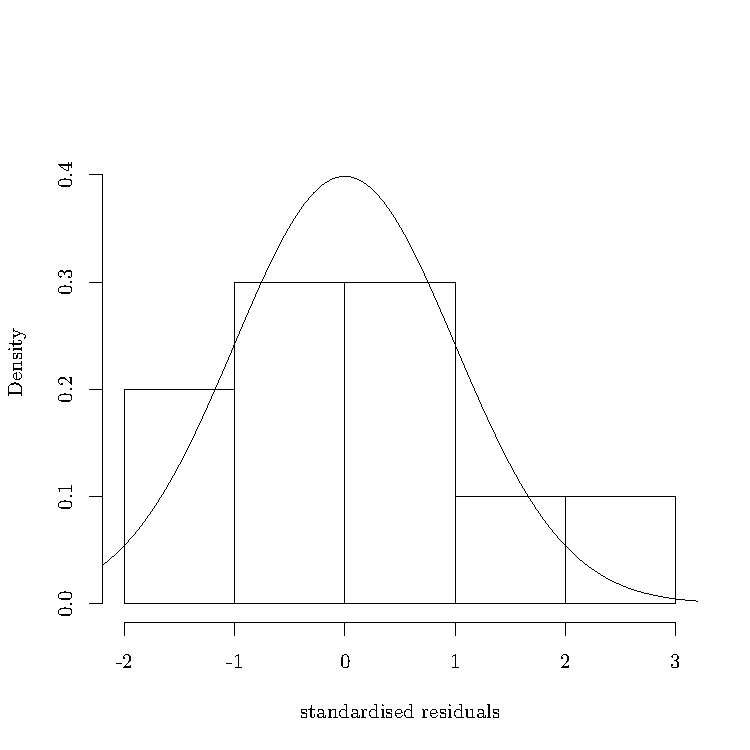
\includegraphics[height=5cm]{figures/R/VALID_crossvalhist} \qquad
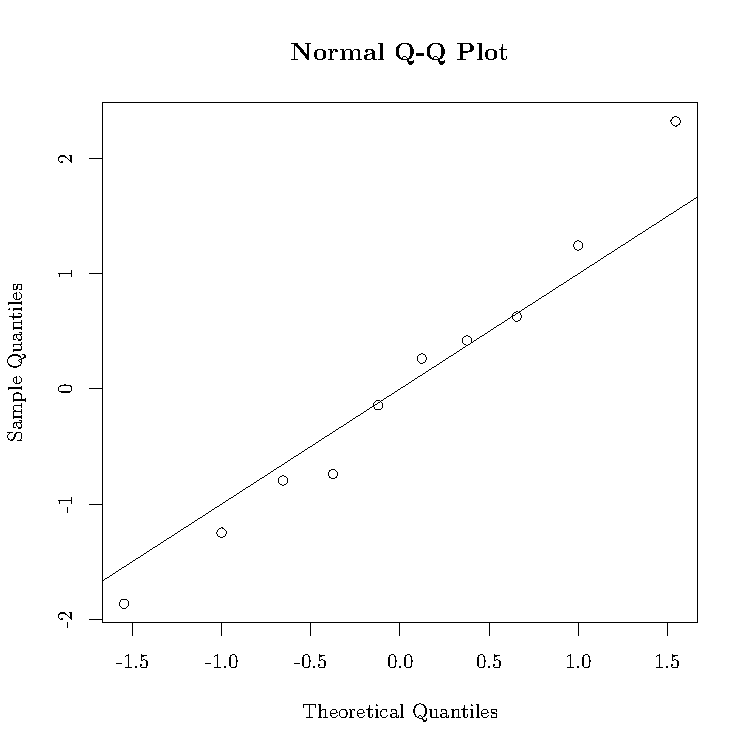
\includegraphics[height=5cm]{figures/R/VALID_crossvalqqplot}
\end{center}
\end{frame}

% \end{frame}


%%%%%%%%%%%%%%%%%%%%%%%%%%%%%%%%%%%%%%%%%%%%%%%%%%%%%%%%%%%%%%%%%%%%%%%%%%%%%%%
%%%%%%%%%%%%%%%%%%%%%%%%%%%%%%%%%%%%%%%%%%%%%%%%%%%%%%%%%%%%%%%%%%%%%%%%%%%%%%%
%%%%%%%%%%%%%%%%%%%%%%%%%%%%%%%%%%%%%%%%%%%%%%%%%%%%%%%%%%%%%%%%%%%%%%%%%%%%%%%
%%%%%%%%%%%%%%%%%%%%%%%%%%%%%%%%%%%%%%%%%%%%%%%%%%%%%%%%%%%%%%%%%%%%%%%%%%%%%%%
\end{document}



\structure{}

\begin{center}
  \begin{tabular}{|c|cc|}

  \end{tabular}
\end{center}

###
%%%%%%%%%%%%%%%%%%%%%%%%%%%%%%%%%%%%%%%%%%%%%%%%%%%%%%
\begin{frame}{}

\end{frame}

###
\begin{block}{}

\end{block}

###
\begin{center}
\includegraphics[height=5cm]{figures/}
\end{center}

###
\begin{columns}[c]
\column{5cm}

\column{5cm}

\end{columns}
